%LaTeX file for Physics GRE review

%Preamble
\documentclass[twoside]{article}
\usepackage{calligra}
\usepackage{times}
\usepackage[geometry]{ifsym}
\usepackage[left=5cm,right=5cm, top=3cm,bottom=3cm]{geometry}
\usepackage{array}
\usepackage{hyperref}
\usepackage{graphicx}
\usepackage{multirow}
\usepackage{fancyhdr}
\usepackage{amsmath}

\hypersetup{
    colorlinks,
    citecolor=black,
    filecolor=black,
    linkcolor=blue,
    urlcolor=black
}

\DeclareMathAlphabet{\mathcalligra}{T1}{calligra}{m}{n}
\DeclareFontShape{T1}{calligra}{m}{n}{<->s*[2.2]callig15}{}

%Macros
\newcommand{\scripty}[1]{\ensuremath{\mathcalligra{#1}}}
\newcommand{\scriptr}{\ensuremath{\scripty{r}\hspace{2pt}}}
\newcommand{\dbar}{\ensuremath{\mathchar'26\mkern-12mu d}}
%\newcommand{\christoffel}[3][i]{\ensuremath{\Gamma^{#1#2}_{#3}}} % use: \christoffel[s]{k}{m}

%Document
\begin{document}

\title{A Concise Review of Undergraduate Physics in Preparation for the Physics GRE}
\author{Jeffrey Hetherly}
\date{\today}
\maketitle
\thispagestyle{empty}

\newpage
%Format fancy header and footer
\fancyhf{}
\setlength{\headheight}{15pt}
\pagestyle{fancyplain}
\renewcommand{\headrulewidth}{0.1pt}
\renewcommand{\footrulewidth}{0.1pt}

\fancyhead[CE]{\leftmark}
\fancyhead[CO]{Jeffrey Hetherly}
\fancyfoot[LO, RE]{\thepage}

\setcounter{page}{1}
\pagenumbering{roman}
\setcounter{tocdepth}{3}
\tableofcontents

\newpage
%\section*{Introduction}
%Format fancy header and footer
\fancyhf{}
\setlength{\headheight}{15pt}
\pagestyle{fancyplain}
\renewcommand{\headrulewidth}{0.1pt}
\renewcommand{\footrulewidth}{0.1pt}

\fancyhead[CO]{\leftmark}
\fancyhead[CE]{Jeffrey Hetherly}
\fancyfoot[LE, RO]{\thepage}

\pagenumbering{arabic}
\setcounter{page}{1}
\section{Introduction}

This document is intended for those studying for the GRE subject test in physics.
It should be used alongside various undergraduate texts as a sort of guide and it does not contain any sample problems.
As such, the available practice exams (four as of the writing of this document: GR8677, GR9277, GR9677, and GR0177) and the web site \texttt{http://grephysics.net/} are invaluable resources in preparing for the exam.
Another great resource is the Ohio State SPS website.
They have ``minitests'' that are categorized by subject so you can practice certain subjects individually and links to the available practice exams.
The vast majority of the Physics GRE (or PGRE as it will be referred to from now on) questions are sophomore and junior physics undergraduate level (in other words, one should be able to answer most of the questions on the exam by end of the junior year).
A two month study period should be sufficient for most physics students to make an adequate score.
This gives enough time to review and study the material as well as practice the exams and refine the student's number crunching ability.

The four PGRE tests are vital to understanding what could be asked on future tests.
However, not all of them are equally relevant for current PGRE subject matter.
The earliest one can be used as a great ``warmup'' test, but many test takers (myself included) don't feel that it is an accurate representation of the current test.
I personally used it at the beginning of my two-month study period but eventually dropped it from my routine by the last two weeks.
The middle two tests are better practice for your arithmetic skills (GR9677 is a beast).
The most current practice test is obviously the best representation of the current test.
GR0177 is not nearly as intense as GR9677 but still requires a large breadth of physics knowledge and a decent amount of arithmetic skill.
I saved practicing this one for my last three weeks.
By the end of week six I could do all 399 problems on the four tests and score a 990 during my practice runs.
However, my actual score wasn't nearly as impressive.

The review covers key material in classical mechanics, electricity and magnetism, optics and wave phenomena, quantum mechanics, thermodynamics, statistical mechanics, modern physics (including special relativity, atomic physics, etc\ldots), and some useful mathematical information.
This review is not limited to simply what is found in the practice exams.
It contains additional information intended to prepare the reader for exam questions that \emph{could} be asked.
Work as many problems on these subjects as possible and understand every question in the PGRE practice tests.

I tried to keep a consistent notation throughout the whole document, but when covering most of undergraduate physics I ran into several conflicting conventions in notation (i.e. \(P\) for pressure, power, and momentum).
I hope this doesn't cause confusion, but I wanted to stick to how things are commonly referred to and I feel that their meaning is obvious in context.


\newpage
\section{Classical Mechanics}

The following subsections cover the basic knowledge needed for the classical mechanics questions on the exam.
The first subsection simply provides a quick reference for essential equations.
However, simply stating conservation of momentum is no substitute for actually working out several problems using conservation of momentum.
As such, the fist section is deceptively concise.
Most of the time studying this section should be spent brushing up on skills to use equations from the Basic Mechanics subsection.
The second subsection is over Lagrangian and Hamiltonian mechanics and reviews the basic equations involved.
There is no substitute for constructing the kinetic energy and potential energy in terms of generalized coordinates for yourself.
The subsequent subsections go into more detail about topics such as gravitation, normal modes, and mechanical waves.
An excellent quantitative and qualitative understanding of this section is necessary for the PGRE.

\subsection{Basic Mechanics}

\subsubsection{Translational and Rotational Kinematics}

The following are derived from:\\
\( \mathbf{a} = \mathrm{const.} \),  \(a = \frac{\mathrm{d}v}{\mathrm{d}t} =  v\frac{\mathrm{d}v}{\mathrm{d}x}  \),  \( v=\frac{\mathrm{d}x}{\mathrm{d}t} \)\\
\(  \vec{\alpha} = \mathrm{const.} \),  \(\alpha = \frac{\mathrm{d}\omega}{\mathrm{d}t} =  \omega\frac{\mathrm{d}\omega}{\mathrm{d}\theta}  \),  \( \omega=\frac{\mathrm{d}\theta}{\mathrm{d}t} \)
\begin{itemize}
\item \( \Delta s = v_0 t + \frac{1}{2} a t^{2} \)
\item \( \Delta v = a t \)
\item \( v^2 -  v_0^2 =  2a \Delta s \)
\item \( \Delta \theta = \omega_0 t + \frac{1}{2} \alpha t^{2} \)
\item \( \Delta \omega = \alpha t \)
\item \(  \omega^2 -   \omega_0^2 =  2\alpha \Delta \theta \)
\end{itemize}
Projectile motion:\\* \( y_{max}=\frac{v_0^2 \sin^2(\theta)}{2g} \)\\* \( x_{max}=\frac{v_0^2 \sin(2\theta)}{g} \)\\\\*
Circular motion:\\* \(s_{arc}=R\theta\)\\* \( v_{tangential}=R\omega \)\\* \(a_{centripetal}=\frac{v_{tangential}^2}{R}=R\omega^2\)\\* \( a_{tangential}=R\alpha \)

\subsubsection{Rotations}
Moment of Inertial (for symmetric bodies): \(I=\sum_im_i(r_{\bot})_i^2 \to \int r_{\bot}^2\,dm\)\\*
(\(r_{\bot}\) is the perpendicular distance from the axis of rotation)
\newpage
Common moments of inertial:
\begin{center}
 
\includegraphics[scale=0.5]{images/PGRE_Figures_1p1p2_Ring.png}
 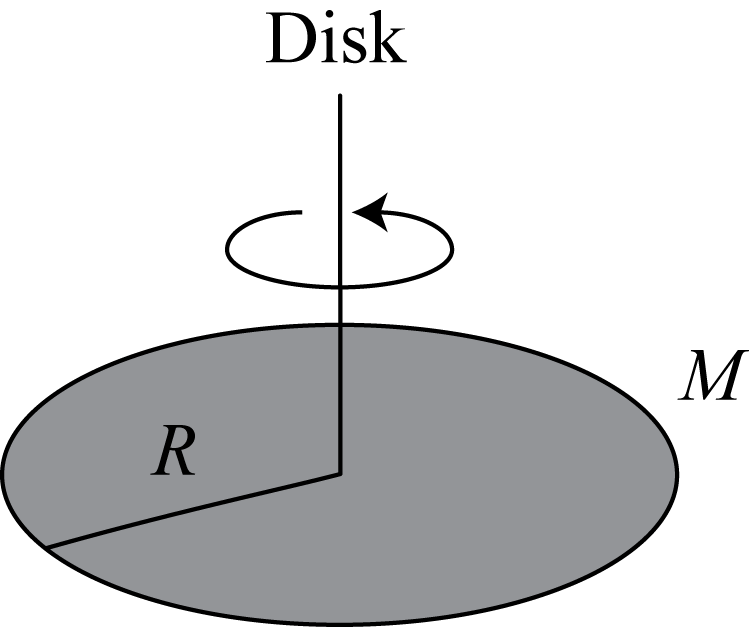
\includegraphics[scale=0.5]{images/PGRE_Figures_1p1p2_Disk.png}
 
\includegraphics[scale=0.5]{images/PGRE_Figures_1p1p2_Rod.png}
 \end{center}
\begin{itemize}
\item Ring: \(I=MR^2\)
\item Disk: \(I=\frac{1}{2}MR^2\)
\item Rod: \(I=\frac{1}{12}ML^2\)
\item Solid Sphere: \(I=\frac{2}{5}MR^2\)
\item Spherical Shell: \(I=\frac{2}{3}MR^2\)
\end{itemize}
Know which dimensions are important for calculating moments of intertial.
(e.g.: A cylinder of length \(L\) that rotates about its length has the same moment of inertial as a disk rotating about the same axis.)\\*
Derivation of \(I\) for a solid sphere: \\*
(Slice sphere into thin disks of radius \(R_{\bot}\) and thickness \(\mathrm{d}z\))
\begin{eqnarray}
\mathrm{d}I_{disk}&=&\frac{1}{2}R_{\bot}^2\mathrm{d}m \nonumber \\
\mathrm{d}m &=& \rho\pi R_{\bot}^2\mathrm{d}z \nonumber \\
I_{sphere}=\int_{-R}^{R}\frac{1}{2}\pi\rho R_{\bot}^4\mathrm{d}z &=& \int_{-R}^{R}\frac{1}{2}\pi\rho (R^2-z^2)^2\mathrm{d}z \nonumber \\
I_{sphere}=\frac{8}{15}\pi\rho R^5 &=& \frac{2}{5}MR^2 \nonumber
\end{eqnarray}
Parallel axis theorem: \(I=I_{CM}+Md^2\)\\*
Radius of Gyration: \(R_{gyration}=\sqrt{I/M}\)\\\\*
Review rolling without slipping.\\\\*
Torque: \(\vec{\tau}=\mathbf{r}\times\mathbf{F}\)\\*
Angular Momentum: \(\mathbf{L}=\mathbf{r}\times\mathbf{p}=I\vec{\omega}\)

\subsubsection{Momenta}
\(\mathbf{p}=m\mathbf{v}\)\\*
\(\mathbf{L}=\mathbf{r}\times\mathbf{p}\)\\\\*
Both \( \mathbf{p} \) and \( \mathbf{L} \) are conserved if there are no external forces acting on the bodies.\\*
\(\Delta \mathbf{p}=\mathbf{p}_f-\mathbf{p}_i=0\)\\*
\(\Delta \mathbf{L}=\mathbf{L}_f-\mathbf{L}_i=0\)

\subsubsection{Newton's Second Law}
\( \displaystyle\sum_{i}\mathbf{F_{\mathit{i}}}=\frac{\mathrm{d}\mathbf{p}}{\mathrm{d}t} \) \(\to\) \( \displaystyle\sum_{i}\mathbf{F_{\mathit{i}}}=m\mathbf{a} \) when \(\mathit{m} = \mathrm{const.}\)\\*
\( \displaystyle\sum_{i}\vec{\tau}_{\mathit{i}}=\frac{\mathrm{d}\mathbf{L}}{\mathrm{d}t} \) \(\to\) \( \displaystyle\sum_{i}\vec{\tau}_{\mathit{i}}=I\vec{\alpha} \) when \(I = \mathrm{const.}\)\\\\*
Statics:\\*
\( \displaystyle\sum_{i}\mathbf{F_{\mathit{i}}}=m\mathbf{a} =\vec{0}\)\\*
\( \displaystyle\sum_{i}\vec{\tau}_{\mathit{i}}=I\vec{\alpha} =\vec{0}\)\\\\*
Frictional force:\\*
\( F_{fric}=\mu N \)  where \(N\) is the normal force on the object\\\\*
Pulleys:
\begin{center}

\includegraphics[scale=0.5]{images/PGRE_Figures_1p1p4_Pulleys.png}
\end{center}
\begin{enumerate}
\item Tension is uniform throughout the rope.
\item When the rope is anchored to a support the pulley system acts as a force multiplier.
\end{enumerate}

\subsubsection{Fictitious Forces}
\(\mathbf{F}'=\mathbf{F}_{physical}-m\mathbf{A}_0-2m\vec{\omega}\times \mathbf{v}'-m\dot{\vec{\omega}}\times \mathbf{r}'-m\vec{\omega}\times\left( \vec{\omega}\times\mathbf{r}' \right)\)\\\\*
\(\mathbf{F}_{physical}\) are any true forces from an inertial perspective\\*
\(\mathbf{A}_0\) is the acceleration of the entire frame\\*
\(\mathbf{F}_{Coriolis}=-2m\vec{\omega}\times \mathbf{v}'\)\\*
\(\mathbf{F}_{transverse}=-m\dot{\vec{\omega}}\times \mathbf{r}'\)\\*
\(\mathbf{F}_{centrifugal}=-m\vec{\omega}\times\left( \vec{\omega}\times\mathbf{r}' \right)\)\\\\*
At Earth's surface:\\*
\(\mathbf{F}_{transverse}=\mathbf{0}\)\\*
\(\mathbf{F}_{centrifugal}\approx\mathbf{0}\)\\*
\(m\mathbf{g}_0-m\mathbf{A}_0=m\mathbf{g}\)\\\\*
Therefore, \(\mathbf{F}'=\mathbf{F}_{physical}+m\mathbf{g}-2m\vec{\omega}\times \mathbf{v}'\)\\\\*
If one defines a coordinate system where \(\hat{x}'\) is "east," \(\hat{y}'\) is "north," and \(\hat{z}'\) is "vertical," then \(\vec{\omega}=\omega\cos{\lambda}\hat{y}'+\omega\sin{\lambda}\hat{z}'\) (where \(\lambda\) is the latitude)

\subsubsection{Work and Energy}
Work-Kinetic Energy Theorem:\\*
\(\displaystyle W_{trans}=\int \mathbf{F}\cdot\,\mathrm{d}\mathbf{s}=\Delta K_{trans}\)\\*
\(\displaystyle W_{rot}=\int \tau\,\mathrm{d}\theta=\Delta K_{rot}\)\\*
\(K_{trans}=\frac{1}{2}mv^2\)\\*
\(K_{rot}=\frac{1}{2}I\omega^2\)\\\\*
Potential Energies:\\*
\(U_{gravity}=mgh\)\\*
\(U_{spring}=\frac{1}{2}kx^2\)\\
In general (for a conservative force \(\nabla\times\mathbf{F}=0\)): \(\mathbf{F}=-\nabla\cdot U\)\\\\*
Conservation of energy can only be used in special circumstances:\\*
\(\Delta E=E_f-E_i=K_f+U_f-(K_i+U_i)=0\)\\\\*
Energy Dissipated Through a Frictional Force: \(E_{lost}=\mu F_Nd\)

\subsubsection{Power and Impulse}
Power:\\*
\(P=\frac{\mathrm{d}W}{\mathrm{d}t} \)\\*
\( P=\mathbf{F}\cdot\mathbf{v}\) when \( \mathbf{F}=\mathrm{const.} \)\\*
\( P=\tau\omega\) when \( \vec{\tau}=\mathrm{const.} \)\\\\*
Impulse:\\*
\(I=\Delta p=\int F\,\mathrm{d}t\)\\*
\(H=\Delta L=\int \tau\,\mathrm{d}t\)

\subsubsection{Collisions}
In general, use conservation and momentum and energy for non-relativistic collisions.\\*
\(\Delta \mathbf{p}=0\) for both elastic and inelastic collisions\\*
\(\Delta \mathbf{L}=0\) for both elastic and inelastic collisions\\*
\(\Delta E=0\) only for elastic collisions\\\\*
Linear Elastic Collisions (no rotation or interaction potential):\\*
Factoring the kinetic energy and dividing by the momentum yields these two equations\\*
\( v_{1i} + v_{1f} = v_{2i} + v_{2f} \)\\*
\(m_1 v_{1i}+m_2v_{2i}=m_1 v_{1f}+m_2v_{2f}\)

\subsubsection{Many Particle Systems}
Center of Mass for Discrete Particles: \(\displaystyle \mathbf{r}_{CM}=\frac{\sum_{i} m_i\mathbf{r}_i}{\sum_{i} m_i}=\frac{\sum_{i} m_i\mathbf{r}_i}{M}\)\\*
Components:\\*
\(x_{CM}=\frac{\sum_{i} m_i x_i}{M}\)\\*
\(y_{CM}=\frac{\sum_{i} m_i y_i}{M}\)\\*
\(z_{CM}=\frac{\sum_{i} m_i z_i}{M}\)\\\\*
 Center of Mass for a Continuous Mass Distribution:\\*
 \(x_{CM}=\frac{\int_{V} \rho x\mathrm{d}V}{M}\)\\*
 \(y_{CM}=\frac{\int_{V} \rho y\mathrm{d}V}{M}\)\\*
 \(z_{CM}=\frac{\int_{V} \rho z\mathrm{d}V}{M}\)\\\\*
 Total momentum: \(\mathbf{p}_{CM}=M\mathbf{v}_{CM}\)\\*
 Total angular momentum: \(\displaystyle\mathbf{L}=\mathbf{r}_{CM}\times M\mathbf{v}_{CM} + \sum_{i}\bar{\mathbf{r}}_i \times M\bar{\mathbf{v}}_i\)\\*
 where \(\bar{\mathbf{r}}_i = \mathbf{r}_i-\mathbf{r}_{CM}\) and \(\bar{\mathbf{v}}_i = \mathbf{v}_i-\mathbf{v}_{CM}\)\\\\*
 The Rocket Equation: \(m\dot{\mathbf{v}}=\mathbf{F}_{ext}+\dot{m}\mathbf{v}_{rel}\)\\*
 \(\mathbf{v}_{rel}\) is the velocity of the propellent\\*
 (Note that this is NOT derived from Newton's second law! It's derived from impulse considerations.)

\subsubsection{Fluid Mechanics}
Pressure (force/area):\\*
\(P=\frac{F}{A}\)\\*
Conservation of mass (for incompressible, irrotational fluids) yields\\*
\(A_1v_1=A_2v_2\) where \(A\) is the cross sectional area and \(v\) is the speed of the fluid\\*
Conservation of energy yields (Bernoulli's equation)\\*
\(P_i+\rho_igh_i+\frac{1}{2}\rho_iv_i^2=\mathrm{const.}\) where \(\rho\) is the density of the fluid\\\\*
Review capillary action.

\subsection{Lagrangian \& Hamiltonian Mechanics}
%For this subsection \(K\to T\) and \(U\to V\).

\subsubsection{Lagrangian Mechanics}
The Lagrangian: \(L=L(q_1,\ldots,q_n,\dot{q}_1,\ldots,\dot{q}_n,t)=T-V\)\\*
(Kinetic energy minus the potential energy)\\*
Review generalized coordinates to see how to construct \(T\) and \(V\).\\*
Lagrange's equation: \(\displaystyle\frac{\partial L}{\partial q}=\frac{\mathrm{d}}{\mathrm{d}t}\left(\frac{\partial L}{\partial \dot{q}}\right)\)\\\\*
Lagrange's equation is derived from finding the extremum of the action integral \(\displaystyle S=\int_{t_1}^{t_2}L\,\mathrm{d}t\)

\subsubsection{Forces of Constraint}
Consider a system with \(n\) generalized coordinates and \(m\) equations of constraint \(f_j\)
\begin{eqnarray}
i&=&1,2,\ldots,n \nonumber \\
j&=&1,2,\ldots,m \nonumber \\
f_j(q_i,t) &=& 0 \nonumber \\
\frac{\mathrm{d}}{\mathrm{d}t}\frac{\partial L}{\partial \dot{q}_i}&=&\frac{\partial L}{\partial q_i}+\sum_j\lambda_j(t)\frac{\partial f_j}{\partial q_i} \nonumber
\end{eqnarray}
\(\sum_j\lambda_j(t)\frac{\partial f_j}{\partial q_i}\) is referred to as the force of constraint.

\subsubsection{Hamiltonian Mechanics}
The Hamitonian: \(H=H(q_1,\ldots,q_n,p_1,\ldots,p_n,t)= \sum_{i=1}^{n} p_i\dot{q}_i-L=T+V\)\\*
Hamilton's equations:
\begin{itemize}
\item \(\displaystyle\dot{q}=\frac{\partial H}{\partial p}\)
\item \(\displaystyle\dot{p}=-\frac{\partial H}{\partial q}=\frac{\partial L}{\partial q}\)
\item \(\displaystyle\frac{\partial H}{\partial t}=-\frac{\partial L}{\partial t}\)
\end{itemize}
Another useful relation is \(p=\frac{\partial L}{\partial \dot{q}}\)\\\\*
If \(t\) doesn't explicitly appear in the Lagrangian, then it will not be in the Hamiltonian and the Hamiltonian will be a constant of motion (conservation of energy).\\*
An ignorable (or cyclical) coordinate is one in which does not appear explicitly in the Lagrangian. (e.g. If \(q_n\) is an ignorable coordinate, then \(L=L(q_1,\ldots,q_{n-1},\dot{q}_1,\ldots,\dot{q}_n,t)\))

\subsection{Gravitation}
Newton's law of universal gravitation:\\*
\(\displaystyle\mathbf{F}_{gravity}=-G\frac{m_1m_2}{r_{12}^2}\hat{r}_{12}\)\\*
For an object near the surface of the earth:\\*
\(\mathbf{F}_{gravity}=-mg\hat{e}_r\)

\subsubsection{Kepler's Laws}
\begin{enumerate}
\item All planets' orbits are elliptical in shape. This is due to the inverse square nature of the gravitational force.\\*
Orbits are defined by their eccentricity:
\begin{itemize}
\item \(1<\epsilon\): hyperbolic orbit \(\to\) highest total orbital energy
\item \(\epsilon =1\): circular orbit \(\to\) any perturbation in orbital energy destroys this perfect orbit
\item  \(0<\epsilon < 1\): elliptical orbit \(\to\) most stable closed orbit
\item \(\epsilon = 0\): parabolic orbit \(\to\) has total orbital energy equal to zero
\end{itemize}
\item Each planet's orbit sweeps out an equal amount of area in an equal amount of time. This is due the conservation of angular momentum (\(L=mr^2\dot{\theta}=\mathrm{const.}\)).\\*
\(\frac{\mathrm{d}A}{\mathrm{d}t}=\frac{L}{2m}=\mathrm{const.}\)\\*
\(T_{period}=\frac{A_T}{\frac{\mathrm{d}A}{\mathrm{d}t}}=\frac{2mA_T}{L}\)
\item The square of the period of a planet is directly proportional to cube of its semi-major axis (\( T_{period}^2 \propto a^3\)). This law is easily derived for circular orbits (The law has the same form for elliptical orbits but that derivation is far beyond the scope of the PGRE).\\*
\begin{eqnarray}
\displaystyle\sum F_r=G\frac{Mm}{r^2}&=&ma_{centripetal}=mr\omega^2 \nonumber \\
G\frac{M}{r^3}&=&\left( \frac{2\pi}{T_{period}} \right)^2 \nonumber \\
T_{period}&=&\frac{2\pi}{\sqrt{GM}}r^{3/2}  \nonumber
\end{eqnarray}
In general: \(\displaystyle T_{period}^2=\frac{4\pi^2}{GM}a^{3}\)\\*
This same type of derivation is used to find the orbital speed: \(v=\sqrt{\frac{GM}{r}}\)\\*
Notice that the period and orbital speed are not related to the mass of the orbiting body.\\*
If \(T_{period}\) is given in years and \(a\) is in A.U., then \(T_{period}^2=a^3\)\\*
If one is given information about a planet and its satellite:\\* \(\displaystyle\frac{m_{planet}}{M_{sun}}=\frac{r_{sat}^3T_{planet}^2}{r_{planet}^3T_{sat}^2}\)
\end{enumerate}

\subsubsection{Central Forces and Reduced Mass}
The total energy of an orbit is given by: \(E_T=\frac{1}{2}m\dot{r}^2+U_{eff}\)\\*
\(U_{eff}\) is the effective potential energy of the orbiting body: \(U_{eff}=\frac{L^2}{2mr^2}-\frac{GMm}{r}\)\\*
Virial Theorem: \(\overline{K}=-\frac{1}{2}\overline{\sum_i \mathbf{F}_i\cdot \mathbf{r}_i}\)\\*
If the force is derived from a central potential \(U=br^n\): \(\overline{K}=\frac{n}{2}\overline{U}\)\\*
The total energy for a body in a closed orbit is: \(E_T=\frac{-GMm}{2a}\)\\*
The escape velocity of an object is the speed needed to completely escape the gravitational pull of a massive object.
It can be derived from considering the energy of a mass in a gravitational field:
\begin{eqnarray}
\Delta E&=&0 \nonumber \\
K_i+U_i&=&K_f+U_f\nonumber\\
\frac{1}{2}mv_i^2-\frac{GMm}{r}&=&0\nonumber\\
v_e&=&\sqrt{\frac{2GM}{r}}\nonumber
\end{eqnarray}
If one uses the surface of the Earth as the starting point: \(v_e=\sqrt{2gR_E}\)\\*
Bertrand's theorem: Only two types of potentials can produce stable, closed orbits; the inverse, central potential \(U(r)=\frac{-k}{r}\) and the radial harmonic oscillator \(U(r)=\frac{1}{2}kr^2\)\\\\*
The reduced mass of two bodies moving about their center of mass is \(\mu=\frac{m_1m_2}{m_1+m_2}\)\\*
Replace \(m\) in \(ma_{centripetal}\) with \(\mu\) to get Kepler's 3$^{\mathrm{rd}}$ law: \(T_{period}=\frac{2\pi}{\sqrt{G(m_1+m_2)}}a^{3/2}\)\\*
If \(a\) is in A.U. and \(T_{period}\) is in years, then \(T_{period}=\frac{1}{\sqrt{m_1+m_2}}a^{3/2}\)

\subsubsection{Orbital Equation}
\(l=\frac{L}{m}\) and \(u=\frac{1}{r}\) (where \(L\) is the angular momentum, not the Lagrangian)
\begin{itemize}
\item Conservation of Angular Momentum: \(r^2\dot{\theta}=l\)
\item Orbital Equation: \(\displaystyle\frac{\mathrm{d}^2u}{\mathrm{d}\theta^2}+u+\frac{1}{ml^2u^2}f(u^{-1})=0\)
\end{itemize}
Derivation of orbital equation(s) using Lagrange's equations:
\begin{eqnarray}
x&=&r\cos{\theta}  \nonumber \\
\dot{x}&=&\dot{r}\cos{\theta}-r\dot{\theta}\sin{\theta} \nonumber \\
y&=&r\sin{\theta} \nonumber \\
\dot{y}&=&\dot{r}\sin{\theta}+r\dot{\theta}\cos{\theta} \nonumber \\
T = \frac{1}{2}m(\dot{x}^2+\dot{y}^2) &=& \frac{1}{2}m(\dot{r}^2+r^2\dot{\theta}^2) \nonumber \\
L&=& \frac{1}{2}m(\dot{r}^2+r^2\dot{\theta}^2) - V(r) \nonumber
\end{eqnarray}
\(\theta\) is an ignorable coordinate
\begin{eqnarray}
\frac{\partial L}{\partial \theta}&=&0 \nonumber \\
\frac{\mathrm{d}}{\mathrm{d}t}\frac{\partial L}{\partial \dot{\theta}}&=&\frac{\mathrm{d}}{\mathrm{d}t}(mr^2\dot{\theta})  \nonumber
\end{eqnarray}
Hence, \(mr^2\dot{\theta} = const.\)\\*
Remember that \(f(r)=-\frac{\partial V}{\partial r}\)
\begin{eqnarray}
\frac{\partial L}{\partial r}&=&mr\dot{\theta}^2+f(r) \nonumber \\
\frac{\mathrm{d}}{\mathrm{d}t}\frac{\partial L}{\partial \dot{r}}&=&m\ddot{r}  \nonumber \\
m\ddot{r}&=&mr\dot{\theta}^2+f(r)  \nonumber \\
m\ddot{r}&=&m\frac{l^2}{r^3}+f(r)  \nonumber
\end{eqnarray}
Using \(\dot{r}=-l\frac{\mathrm{d}u}{\mathrm{d}\theta}\) and \(\ddot{r}=-u^2l^2\frac{\mathrm{d}^2u}{\mathrm{d}\theta^2}\)
\begin{eqnarray}
\frac{\mathrm{d}^2u}{\mathrm{d}\theta^2}&=&-u-\frac{1}{ml^2u^2}f(u^{-1}) \nonumber
\end{eqnarray}

\newpage

\subsection{Periodic Motion}
Angular frequency of small oscillations for various objects
\begin{itemize}
\item Physical pendulum: \(\omega_p=\sqrt{\frac{Mgd}{I}}\) where \(d\) is the distance from the support to the center of mass
\item Ideal pendulum (let \(d \to l\) and \(I \to Ml^2\)): \(\omega_p=\sqrt{\frac{g}{l}}\)
\item Mass on a spring: \(\omega_s=\sqrt{\frac{k}{m}}\)
\item In general: \(\omega=\sqrt{\frac{V_0''}{M}}\)\\*
\(V_0''\) is the second derivative of the potential energy evaluated at \(q=0\) (equilibrium).
\end{itemize}

\subsubsection{Simple Harmonic Motion}
Governing equation: \(\ddot{x}=-\omega_s^2x\)\\*
Solution: \(x(t)=A\sin(\omega_st-\phi)\)\\*
Total energy in a simple harmonic oscillator (SHO): \(E_T=\frac{1}{2}kA^2=\frac{1}{2}m\omega_s^2A^2\)\\*
Conservation of energy gives the speed of the mass \(v=\omega_s\sqrt{A^2-x^2}\)\\*
This only becomes obvious when studying capacitors: \(k_{parallel}=\sum_i k_i\) and \(\frac{1}{k_{series}}=\sum_i \frac{1}{k_i}\)\\*
Torsional pendulum: \(\tau=-\kappa\theta \to T_{period}=2\pi\sqrt{\frac{I}{\kappa}}\)

\subsubsection{Damped Harmonic Motion}
Governing equation: \(\ddot{x}=-2\gamma\dot{x}-\omega_s^2x\)\\*
Solution: \(x(t)=A_1e^{-(\gamma-q)t}+A_2e^{-(\gamma+q)t}\) where \(q=\sqrt{\gamma^2-\omega_s^2}\)\\*
The rate of energy loss in \emph{any} damped oscillator is \(\frac{\mathrm{d}E_T}{\mathrm{d}t}=-2m\gamma\dot{x}^2\)\\*
Total energy in a \emph{weakly} damped oscillator: \(E(t)=\frac{1}{2}m\omega_s^2A^2e^{-t/\tau}=E_0e^{-t/\tau}\)\\\\*
\(q\) determines how damped the system is
\begin{itemize}
\item \(0<q\): Overdamping \(\to\) ``oscillator'' will slowly return to equilibrium
\item \(q=0\): Critical damping \(\to\) \(x(t)=Ate^{-\gamma t}+Be^{-\gamma t}\)
\item \(q\in\Im\): Underdamping \(\to\) \(x(t)=Ae^{-\gamma t}\sin(\omega_dt+\phi)\) where \(\omega_d=\sqrt{\omega_s^2-\gamma^2}\)
\end{itemize}
The quality factor for a weakly damped oscillator is \(Q=\frac{\omega_d}{2\gamma}\)

\subsubsection{Forced Oscillation}
Governing equation: \(\ddot{x}=-2\gamma\dot{x}-\omega_s^2x+F_0\)\\*
Steady-state solution: \(\displaystyle A=\frac{F_0/m}{\sqrt{\left(\omega^2-\omega_s^2\right)^2+\left(\frac{\gamma\omega}{m}\right)^2}}\)\\\\*
When \(\omega\approx\omega_s\) the amplitude increases dramatically. This phenomenon is know as resonance and \(\omega_s\) is the resonant (angular) frequency. At resonance the applied force is in phase with the velocity and the power transferred to the oscillator is maximal. This is analogous the AC driven LRC circuit resonant (angular) frequency.

\subsubsection{General Oscillating Systems}
Assume system has a potential \(V(q_1,q_2,\ldots,q_n)\)\\*
Equilibrium is found when \(\displaystyle\frac{\partial V}{\partial q_i}=0\) with \(i=1,2,\ldots,n\)\\*
Make sure you construct the potential so that \(q_i=0\) are the equilibrium coordinates (This allows the series expansion of \(V\) to be conveniently centered around \(q_i=0\)).\\\\*
Functions evaluated at equilibrium will have the following notation: \(\left(\right)_{eq}=\left(\right)_{q_1=q_2=\ldots=q_n=0}\)\\\\*
For 1-D motion:\\*
\(V(q)\approx\frac{q^2}{2}V_0''\) where \(\displaystyle V_0''=\left(\frac{\mathrm{d}^2V}{\mathrm{d}q^2}\right)_{eq}\)\\*
Stability:
\begin{itemize}
\item Stable: \(V_0'' > 0\)
\item Unstable: \(V_0'' < 0\)
\item Indeterminate: \(V_0'' = 0\)
\end{itemize}
Force is then linear in \(q\): \(F(q)\approx-qV_0''\)\\\\*
Oscillations of bound systems with one degree of freedom:
\begin{eqnarray}
L=T-V&=&\frac{1}{2}(M)_{eq}\dot{q}^2-\frac{1}{2}V_0''q^2 \nonumber
\end{eqnarray}
Taking the appropriate derivatives:
\begin{eqnarray}
(M)_{eq}\ddot{q}&=&-V_0''q  \nonumber\\
\omega&=&\sqrt{\frac{V_0''}{(M)_{eq}}}  \nonumber
\end{eqnarray}
\\*
For \(n\)-D motion:\\*
\(V(q_1,q_2,\ldots,q_n)\approx\frac{1}{2}(K_{11}q_1^2+2K_{12}q_1q_2+K_{22}q_2^2+\ldots)\) where \(\displaystyle K_{ij}=\left(\frac{\partial^2 V}{\partial q_i\partial q_j}\right)_{eq}\)\\\\*
For oscillations about equilibrium:\\*
\begin{eqnarray}
\displaystyle L&=&\frac{1}{2}\sum_{k=1}^{n}\sum_{j=1}^{n}\left(\left(M_{jk}\right)_{eq}\dot{q}_j\dot{q}_k-K_{jk}q_jq_k\right) \nonumber
\end{eqnarray}
The \(n\) equations of motion (denoted by \(k\)) are given by:
\begin{eqnarray}
\displaystyle \sum_{j=1}^{n}\left(\left(M_{jk}\right)_{eq}\ddot{q}_j+K_{jk}q_j\right)&=&0 \nonumber\\
M\ddot{\mathbf{q}}+K\mathbf{q}&=&0\nonumber
\end{eqnarray}
We now look for solutions of the form: \(\mathbf{q}=\mathbf{a}\cos{\omega t}\)\\*
\(\left(K-\omega^2M\right)\mathbf{a}=\mathbf{0}\) must be true\\*
For non-trivial \(\mathbf{a}\):
\begin{eqnarray}
\mathrm{det}\left(K-\omega^2M\right)=0 \nonumber
\end{eqnarray}
This is the equation used to find the \(n\) eigenfrequencies (\(\omega_k\)) of the system.\\\\*
To find the \(\mathbf{a}_k\)'s of the system, plug in \(\omega_k\) into
\begin{eqnarray}
\left(K-\omega_k^2M\right)\mathbf{a}_k=\mathbf{0} \nonumber
\end{eqnarray}
From this you will get a relationship between the components of \(\mathbf{a}_k\).
You can arbitrarily chose the value of the first component, but the convention is to set it to one.\\\\*
The eigenvectors (normal modes) are then given by: \(\mathbf{Q}_k=\mathbf{a}_k\cos{\omega_k t -\delta_k}\)\\\\*
If you can ``guess'' the normal mode \(\mathbf{a}_k\)'s it can greatly simplify the problem (for coupled oscillators there is usually a symmetric and antisymmetric mode).
Consider the matrix whose columns are made of the \(\mathbf{a}_k\)'s:
\begin{eqnarray}
A=\left[\!
  \begin{array}{ c c c c }
       & & &  \\
     \mathbf{a}_1 & \mathbf{a}_2 & \ldots & \mathbf{a}_n \\
      & & &
  \end{array} \!\right] \nonumber
\end{eqnarray}
This matrix will diagonalizes both the \(K\) and \(M\) matrices:
\begin{eqnarray}
K_{diag}&=&A^{\dagger}KA \nonumber\\
M_{diag}&=&A^{\dagger}MA \nonumber
\end{eqnarray}
The eigenfrequencies are then trivial to compute:
\begin{eqnarray}
\omega_k^2&=&\frac{\left[K_{diag}\right]_{kk}}{\left[M_{diag}\right]_{kk}} = \frac{\mathbf{a}_k^{\dagger}K\mathbf{a}_k}{\mathbf{a}_k^{\dagger}M\mathbf{a}_k} \nonumber
\end{eqnarray}

\subsection{Mechanical Waves}

\subsubsection{General Wave Equation}
\(\displaystyle \frac{\partial^2y}{\partial x^2}=\frac{1}{v^2}\frac{\partial^2y}{\partial t^2}\)

\subsubsection{Wave on a String}
Solution for wave on a string: \(y(x,t)=A\sin(kx-\omega t)\) where the wave is moving from left to right\\*
Wave number: \(k=\frac{2\pi}{\lambda}\)\\*
Wave velocity: \(v=\frac{\lambda}{T}=\frac{\omega}{k}=\nu\lambda\)\\*
Wave velocity in terms of material: \(v=\sqrt{\frac{T}{\mu}}\) where \(T\) is the tension in the string and \(\mu\) is the linear mass density\\*
Transverse speed: \(v_y=\frac{\partial y}{\partial t}=-\omega A\cos(kx-\omega t)\)\\*
Transverse acceleration: \(a_y=\frac{\partial^2 y}{\partial t^2}=-\omega^2 y\)\\*
Energy carried in one wavelength: \(E_{\lambda}=\frac{1}{2}\mu\omega^2A^2\lambda\)\\*
Power in one wavelength: \(P_{\lambda}=\frac{E_{\lambda}}{T}=\frac{1}{2}\mu\omega^2A^2v\)\\\\*
Reflection and Transmission (R\&T):\\*
R\&T for waves on a string serve as the archetype for various phenomena.
For the PGRE several questions in optics (phase change due to reflection) and quantum mechanics (nodes of a standing wave and to a lesser extent tunneling) can easily be conceptualized using ideas from R\&T for strings.
Therefore, an effort should be made to understand all the qualitative features of waves on a string.\\*
Important concept: When a wave travels from medium A to medium B and \(v_A>v_B\) (A is less dense than B), it is inverted upon reflection.
Likewise, when a wave travels from B to A, it is \emph{not} inverted.\\*
Review diagrams of R\&T for waves on a string.

\subsubsection{Harmonics}
Superposition of Sinusoidal Waves:\\*
\( y_1=A\sin(kx-\omega t)\) and \( y_2=A\sin(kx-\omega t+\phi)\)\\*
\(y_3=y_1+y_2=2A\cos\left(\frac{\phi}{2}\right)\sin\left(kx-\omega t+\frac{\phi}{2}\right)\)\\\\*
Standing Sinusoidal Wave:\\*
\( y_1=A\sin(kx-\omega t)\) and \( y_2=A\sin(kx+\omega t)\)\\*
\(y_3=y_1+y_2=2A\sin(kx)\cos(\omega t)\)\\*
A node is a point on an \(x\)-\(y\) graph where \(y_3=0\).
The distance between adjacent nodes is \(x=\frac{n}{2}\lambda\) where \(n=0,1,2,\ldots\).
Antinodes are halfway in between nodes.\\\\*
Harmonics:\\*
Harmonics are a set of standing waves for a physical object that when properly combined can recreate any frequency in the object (the eigenvalues for the frequencies).
As far as the PGRE is concerned, one only needs to remember a few key facts:
\begin{itemize}
\item For a system constrained or completely free at both endpoints (string on a guitar, open pipe) the harmonic frequencies are \(f_n=\frac{n}{2L}v\) where \(v\) is the speed of the wave, \(L\) is the length of the string/pipe, and \(n=1,2,\ldots\).
\item For a system constrained at one endpoint (string attached to a movable ring and wall, pipe closed at one end) the harmonic frequencies are \(f_n=\frac{n}{4L}v\).
\item \(f_1\) is called the first harmonic or fundamental frequency.
\item The beat frequency between two harmonics is \(f_{beat}=|f_n-f_m|\).
\end{itemize}
To get the harmonic wavelengths use \(v=\lambda f\).

\subsubsection{Sound Waves}
Speed of Sound (in air): \(v=\sqrt{\frac{B_{modulus}}{\rho}}=331(m/s)\sqrt{1+\frac{T_C}{273^{\circ}\mathrm{C}}}\)\\*
Intensity: \(I=\frac{P}{A}\)\\*
Decibel Scale: \(\beta=10\times\mathrm{log}\left(\frac{I}{I_0}\right)\)\\*
Doppler Effect: \(\displaystyle f_{observed}=\left(\frac{v+v_{observer}}{v+v_{source}}\right)f_{source}\)\\*
(Be consistent with the signs for the velocities.)
\(v\) is the speed of sound, \(v_{observer}\) is the speed of the observer (positive if moving \emph{toward} the source), and \(v_{source}\) is the speed of the source (positive if moving \emph{away} from observer).
Thus, the formula above has the correct signs for an observer and source moving in the same direction.


\newpage
\section{Electricity \& Magnetism}

This section covers material related to the E\&M portion of the exam.
Most of these subsections go into more depth than is required for the PGRE.
Gauss's law, Faraday's law, and radiation originating from charged particles are consistently tested on the practice exams.
Method of images is also something to brush up on.

\subsection{Electrostatics}

\subsubsection{Coulomb's Law}
Force Law: \(\displaystyle\mathbf{F}_E=k_e\frac{q_1q_2}{\scriptr^2}\hat{\scriptr}\)\\\\*
Electric Field:\\*
\(\displaystyle\mathbf{F}_E=q\mathbf{E}\)\\*
\(\displaystyle\mathbf{E}=k_e\sum_i\frac{q_i}{\scriptr_i^2}\hat{\scriptr}_i\to k_e\int\frac{\hat{\scriptr}}{\scriptr^2}\mathrm{d}q\)\\\\*
Electric Field Example: E-field along \(z\)-axis due to a ring of charge \(Q\) centered at the origin and in the \(x\)-\(y\) plane: \(\displaystyle\mathbf{E}=\frac{k_eQd}{(R^2+z^2)^{3/2}}\hat{z}\)

\subsubsection{Gauss's Law}
Electric Flux: \(\Phi_E=\int_S\mathbf{E}\cdot\,\mathrm{d}\mathbf{a}\)\\*
Through a Closed Surface: \(\displaystyle\Phi_E=\oint_{\delta V}\mathbf{E}\cdot\,\mathrm{d}\mathbf{a}\)\\*
Differential Form: \(\nabla\cdot\mathbf{E}=\displaystyle\frac{\rho}{\epsilon_0}\)\\*
Integral Form: \(\displaystyle\oint_{\delta V}\mathbf{E}\cdot\,\mathrm{d}\mathbf{a}=\frac{Q_{enc}}{\epsilon_0}\)\\\\*
Common Uses of Gauss's Law:
\begin{itemize}
\item Spherical Symmetry: Inside uniformly charged sphere of radius \(a \to\) \(\displaystyle E=\frac{k_eQ}{a^3}r=\frac{\rho}{3\epsilon_0}r\)
\item Cylindrical Symmetry: Outside cylinder of radius \(b\) with uniform surface charge \(\to\) \(\displaystyle E=\frac{\sigma b}{\epsilon_0}\frac{1}{r}\)
\item Planar Surface: Near plate with uniform surface charge \(\to\) \(\displaystyle E=\frac{\sigma}{2\epsilon_0}\)
\end{itemize}
Gauss's law is also useful in showing that all the net charge on a conductor must reside on its surface, as well as that there is no E-field inside a conductor and, therefore, no net force on a particle placed in a conductor.\\*
Gauss's law is typically the easiest way to calculate E-fields when enough spatial symmetry is present.

\newpage
\subsubsection{Electric Potential}
\(\nabla\times\mathbf{E}=\vec{0}\to\mathbf{E}=-\nabla V \to -\nabla^2 V=\displaystyle\frac{\rho}{\epsilon_0}\)\\\\*
Electric Potential: \(\displaystyle V(\mathbf{b})-V(\mathbf{a})= -\int_\mathbf{a}^\mathbf{b}\mathbf{E}\cdot\,\mathrm{d}\mathbf{s}\)\\\\*
If \(\mathbf{a}\) is taken to be a reference where \(V(\mathbf{a})=0\), then \(\displaystyle V(\mathbf{r})= -\int_\mathbf{O}^\mathbf{r}\mathbf{E}\cdot\,\mathrm{d}\mathbf{s}\)\\\\*
\(\displaystyle V=k_e\sum_i\frac{q_i}{\scriptr_i} \to k_e\int\frac{\mathrm{d}q}{\scriptr}\)\\*
A conductor is an equipotential and the \(\mathbf{E}\) field is \(\bot\) to the surface just above a conductor (else the surface charge would move).\\*
Electric Potential Example: Potential along \(z\)-axis due to a ring of charge \(Q\) centered at the origin and in the \(x\)-\(y\) plane \(\to\) \(\displaystyle\ V=\frac{k_eQ}{\sqrt{R^2+z^2}}\)

\subsubsection{Electrostatic Force on a Conductor}
Force per unit area: \(\mathbf{f}=\sigma\mathbf{E}_{ave}=\frac{1}{2}\sigma(\mathbf{E}_{above}-\mathbf{E}_{below})\)\\*
(This actually applies to any surface charge.)\\\\*
For a conductor: \(\mathbf{f}=\frac{1}{2\epsilon_0}\sigma^2\hat{\mathbf{n}}\)

\subsubsection{Electric Dipole}
Electric Dipole Moment: \(\mathbf{p}=q\mathbf{d}\) where \(\mathbf{d}\) is the displacement vector pointing from the negative charge (\(-q\)) to the positive charge (\(q\))\\*
\(\displaystyle\mathbf{p}=\int{\mathbf{r'}\rho(\mathbf{r}')\mathrm{d}v'}\)\\\\*
The electric potential from a dipole:\\*
\(\displaystyle V(\mathbf{r})=\frac{1}{4\pi\epsilon_0}=\frac{\mathbf{p}\cdot\hat{\mathbf{r}}}{r^2}\)\\\\*
The field from a dipole:\\*
\(\displaystyle E_{dipole}\propto \frac{p}{r^3}\)\\*
Specifically, \(\displaystyle \mathbf{E}_{dipole}=\frac{1}{4\pi\epsilon_0}\frac{1}{r^3}\left[3\left(\mathbf{p}\cdot\hat{\mathbf{r}}\right)\hat{\mathbf{r}}-\mathbf{p}\right]\)\\\\*
Effect of an external \(\mathbf{E}\) field on a dipole:\\*
Force: \(\mathbf{F}=\left(\mathbf{p}\cdot\nabla\right)\mathbf{E}\)\\*
Torque: \(\vec{\tau}=\mathbf{p}\times\mathbf{E}\)\\*
Potential Energy: \(U=-\mathbf{p}\cdot\mathbf{E}\)

\subsubsection{Dielectrics}
The dipole moment per unit volume is called the polarization \(\mathbf{P}\).\\*
\(\mathbf{P}\cdot\hat{\mathbf{n}}=\sigma_{bound}\)\\*
\(-\nabla\cdot\mathbf{P}=\rho_{bound}\)\\\\*
\(\displaystyle V(\mathbf{r})=\frac{1}{4\pi\epsilon_0}\int{\frac{\hat{\mathbf{\scriptr}}\cdot\mathbf{P}(\mathbf{r}')}{\scriptr^2}\mathrm{d}v'}\)\\\\*
The electric displacement is \(\mathbf{D}=\epsilon_0\mathbf{E}+\mathbf{P}\).\\*
\(\nabla\cdot\mathbf{D}=\rho_{free}\to \displaystyle\oint_{\delta V}\mathbf{D}\cdot\,\mathrm{d}\mathbf{a}=Q_{free_{enc}}\)\\\\*

Linear Dielectrics:\\*
Dielectric Constant: \(\displaystyle\kappa=\frac{\epsilon}{\epsilon_0}\) (note: \(\kappa\geq 1\) typically)\\*
\(\mathbf{P}=(\epsilon-\epsilon_0)\mathbf{E}\)\\*
\(\mathbf{D}=\epsilon\mathbf{E}=\kappa\epsilon_0\mathbf{E}\)\\\\*
A convenient way to calculate \(\displaystyle\sigma_{bound}\) is to use \(\mathbf{D}=\epsilon\mathbf{E}\) with \(\displaystyle\oint_{\delta V}\mathbf{D}\cdot\,\mathrm{d}\mathbf{a}=Q_{free_{enc}}\) to get \(\mathbf{P}\) and finally use the relation \(\mathbf{P}\cdot\hat{\mathbf{n}}=\sigma_{bound}\).

\subsubsection{Energy in an Electrostatic Field}
\(\displaystyle U=\frac{k_e}{2}\sum_j\sum_{i\neq j}\frac{q_iq_j}{r_{ij}} \)\\*
\(\displaystyle U=\frac{\epsilon_0}{2}\int{E^2\mathrm{d}v}\)\\*
\(\displaystyle U=\frac{1}{2}\int{\mathbf{D}\cdot\mathbf{E}\hspace{2pt}\mathrm{d}v}\)

\subsubsection{Method of Images}
Force behaves as if there was an actual image charge present.\\*
Energy, however, needs to be calculated using only regions ``outside'' the conductor. (\(\mathbf{E}=\mathbf{0}\) ``inside'')\\*
For planar conductor, replace the conductor with a mirror image of the charge distribution with opposite charge.\\*
For spherical conductor of radius \(R\), replace the conductor with a charge \(q'\) a distance \(b\) from the origin.
(\(r\) is the distance \(q\) is from the center of the sphere)
\begin{eqnarray}
\displaystyle q'&=&\frac{-R}{r}q \nonumber \\
\displaystyle b&=&\frac{R^2}{r} \nonumber
\end{eqnarray}

\subsubsection{Separation of Variables}
Used to solve Laplace's equation: \(\nabla^2 V(\mathbf{r})=0\)\\\\*
Decompose \(V(\mathbf{r})\) into separate, independent functions of the coordinates.\\\\*
Use boundary conditions to find relationship between the series coefficients and exploit the orthogonality (or orthonormality) of the trigonometric functions, \(P_l\), or \(Y_l^m\).\\\\*
For Cartesian coordinates you must set up and solve each scenario from scratch.\\*
In spherical polar coordinates with azimuthal symmetry, use:\\*
\(\displaystyle V(r,\theta)=\sum_{l=0}^\infty\left(A_lr^l+\frac{B_l}{r^{l+1}}\right)P_l(\cos{\theta})\)

\subsection{Magnetostatics}

\subsubsection{Current}
\(\displaystyle I=\frac{\mathrm{d}q}{\mathrm{d}t}\)\\\\*
Drift Velocity of Charge Carriers: \(I=nqv_DA\)\\*
Current Density: \(J=\frac{I}{A}=nqv_D\to \mathbf{J}=nq\mathbf{v}_D\)\\\\*
Linear Current: \(\mathbf{I}=\lambda \mathbf{v}\)\\*
Surface Current: \(\mathbf{K}=\sigma \mathbf{v}\)\\*
Volume Current: \(\mathbf{J}=\rho \mathbf{v}\)

\subsubsection{Biot-Savart's Law}
\(\displaystyle\mathbf{B}=\frac{\mu_0}{4\pi}\int\frac{\mathbf{I}\times\hat{\scriptr}}{\scriptr^2}\mathrm{d}s'\)\\\\*
\(\displaystyle\mathbf{B}=\frac{\mu_0}{4\pi}\int\frac{\mathbf{K}\times\hat{\scriptr}}{\scriptr^2}\mathrm{d}a'\)\\\\*
\(\displaystyle\mathbf{B}=\frac{\mu_0}{4\pi}\int\frac{\mathbf{J}\times\hat{\scriptr}}{\scriptr^2}\mathrm{d}v'\)\\\\*
Common Uses of Biot-Savart's Law:
\begin{itemize}
\item Circular wire arc at center of curvature: \(\displaystyle B=\frac{\mu_0I\theta}{4\pi R}\)
\item Circular current loop along axis: \(\displaystyle B=\frac{\mu_0I}{2}\frac{r^2}{\left(R^2+z^2\right)^{3/2}}\)
\end{itemize}
Both of these give \(\displaystyle B=\frac{\mu_0I}{2R}\) at the center of a current loop.
Far away from the loop (along the axis) the B-field behaves like \(\displaystyle B\propto\frac{1}{z^3}\).

\subsubsection{Amp\`ere's Law}
DifferentialForm: \(\nabla\times\mathbf{B}=\mu_0\mathbf{J}\)\\*
Integral Form: \(\displaystyle\oint_{\delta S}\mathbf{B}\cdot\,\mathrm{d}\mathbf{l}=\mu_0 I_{enc}\)\\\\*
Common Uses of Amp\`ere's Law:
\begin{itemize}
\item Long wire: \(\displaystyle B=\frac{\mu_0I}{2\pi r}\)
\item Solenoid/Toroid: \(\displaystyle B=\mu_0 n I\) where \(\displaystyle n=\frac{N_{turns}}{l}\) for a solenoid and \(\displaystyle\frac{N_{turns}}{2\pi R}\) for a toroid
\end{itemize}

\subsubsection{Magnetic Forces on Objects}
Particle: \(\mathbf{F}_B=q\mathbf{v}\times\mathbf{B}\)\\*
Wire:  \(\mathbf{F}_B=I\mathbf{L}\times\mathbf{B}\) (\(\mathbf{L}\) connects \emph{endpoints} of wire)\\*
The net magnetic force acting on any closed current loop in \emph{uniform} magnetic field is zero (\(\mathbf{L}=\mathbf{0}\)), but the torque isn't necessarily zero.\\*
\(\vec{\tau}=I\mathbf{A}\times\mathbf{B}\) where \(\mathbf{A}\) is the area enclosed by the loop\\\\*
\(\mathbf{F}=\int I(\mathrm{d}\mathbf{s}\times\mathbf{B})\)\\*
\(\mathbf{F}=\int (\mathbf{K}\times\mathbf{B})\mathrm{d}a\)\\*
\(\mathbf{F}=\int (\mathbf{J}\times\mathbf{B})\mathrm{d}v\)\\\\*
Cyclotron (angular) frequency:
\begin{eqnarray}
ma&=&qvB \nonumber\\
m\omega^2R&=&q\omega RB \nonumber\\
\omega_{cyclotron}&=&\frac{qB}{m} \nonumber
\end{eqnarray}
Force per length between two current carrying wires separated by a distance \(a\): \(\displaystyle\frac{F_B}{l}=\frac{\mu_0I_1I_2}{2\pi a}\) (currents in the same direction attract while opposite currents repel)

\subsubsection{Magnetic Flux}
\(\Phi_B=\int_S\mathbf{B}\cdot\,\mathrm{d}\mathbf{a}\)\\\\*
\(\displaystyle\Phi_B=\oint_{\delta V}\mathbf{B}\cdot\,\mathrm{d}\mathbf{a}=0\to\nabla\cdot\mathbf{B}=\mathbf{0}\)\\*
This last statement just means there are no magnetic monopoles, or ``magnetic charges.''

\subsubsection{Magnetic Vector Pontential}
\(\nabla\cdot\mathbf{B}=\mathbf{0}\to\mathbf{B}=\nabla\times\mathbf{A}\)\\*
\(\nabla^2\mathbf{A}=-\mu_0\mathbf{J}\)\\\\*
\(\displaystyle\mathbf{A}=\frac{\mu_0}{4\pi}\int\frac{I}{\scriptr}\mathrm{d}\mathbf{s}'\)\\\\*
\(\displaystyle\mathbf{A}=\frac{\mu_0}{4\pi}\int\frac{\mathbf{K}(\mathbf{r}')}{\scriptr}\mathrm{d}a'\)\\\\*
\(\displaystyle\mathbf{A}=\frac{\mu_0}{4\pi}\int\frac{\mathbf{J}(\mathbf{r}')}{\scriptr}\mathrm{d}v'\)

\subsubsection{Magnetic Dipole}
\(\mathbf{m} =\int I\mathrm{d}\mathbf{a}\)\\\\*
The magnetic vector potential from a dipole:\\*
\(\displaystyle\mathbf{A}_{dipole}=\frac{\mu_0}{4\pi}\frac{\mathbf{m}\times\hat{\mathbf{r}}}{r^2}\)\\\\*
The field from a dipole:\\*
\(\displaystyle \mathbf{B}_{dipole}=\frac{\mu_0}{4\pi}\frac{1}{r^3}\left[3\left(\mathbf{m}\cdot\hat{\mathbf{r}}\right)\hat{\mathbf{r}}-\mathbf{m}\right]\)\\\\*
Effect of an external \(\mathbf{B}\) field on a dipole:\\*
Force: \(\mathbf{F}=\nabla(\mathbf{m}\cdot\mathbf{B})\)\\*
Torque: \(\vec{\tau}=\mathbf{m}\times\mathbf{B}\)\\*
Potential Energy: \(U=-\mathbf{m}\cdot\mathbf{B}\)

\subsubsection{Dia-Para-Ferromagnetic Materials}
The magnetic dipole moment per unit volume is called the magnetization \(\mathbf{M}\).\\*
\(\nabla\times\mathbf{M}=\mathbf{J}_{bound}\)\\*
\(\mathbf{M}\times\hat{\mathbf{n}}=\mathbf{K}_{bound}\)\\\\*
\(\displaystyle\mathbf{A}(\mathbf{r})=\frac{\mu_0}{4\pi}\int\frac{\mathbf{M}\times\hat{\scriptr}}{\scriptr^2}\mathrm{d}v'\)\\\\*
\(\displaystyle\mathbf{H}=\frac{1}{\mu_0}\mathbf{B}-\mathbf{M}\)\\\\*
\(\nabla\times\mathbf{H}=\mathbf{J}_{free}\)\\*
\(\displaystyle\oint\mathbf{H}\cdot\mathrm{d}\mathbf{l}=I_{free_{enc}}\)\\\\*
For Linear Materials: \(\mathbf{H}=\mu\mathbf{B}\)
\begin{itemize}
\item Diamagnets: \(\mu < \mu_0\to\) no unpaired electrons and field is reduced by Lenz's law acting on electron orbits
\item Paramagnets: \(\mu > \mu_0\to\) has some unpaired electrons that align with applied field
\item Ferromagnets: \(\mu \gg \mu_0\to\) has many unpaired electrons and forms magnetic domains within the material
\end{itemize}

\subsection{Electrodynamics}

\subsubsection{Displacement Current and the Amp\`ere-Maxwell Law}
\(\displaystyle I_d=\epsilon_0\frac{\mathrm{d}\Phi_E}{\mathrm{d}t}=\epsilon_0\frac{\mathrm{d}}{\mathrm{d}t}\int_S\mathbf{E}\cdot\,\mathrm{d}\mathbf{a}\)\\*
\(\displaystyle\oint_{\delta S}\mathbf{B}\cdot\,\mathrm{d}\mathbf{l}=\mu_0 (I+I_d)=\mu_0I +\mu_0\epsilon_0\frac{\mathrm{d}\Phi_E}{\mathrm{d}t}\)\\*
\(\displaystyle\nabla\times\mathbf{B}=\mu_0\mathbf{J}+\mu_0\epsilon_0\frac{\partial\mathbf{E}}{\partial t}\)

\subsubsection{Lorentz Force}
\(\mathbf{F}_L=q(\mathbf{E}+\mathbf{v}\times\mathbf{B})\)

\subsubsection{Faraday's Law}
\(\displaystyle{\cal{E}}_{induced}=-\frac{\partial\Phi_B}{\partial t}\)\\\\*
\(\displaystyle\nabla\times\mathbf{E}=-\frac{\partial\mathbf{B}}{\partial t}\)\\\\*
\(\displaystyle\oint\mathbf{E}\cdot\mathrm{d}\mathbf{l}=\frac{-\mathrm{d}\Phi_B}{\mathrm{d}t}\)\\\\*
Example: Induced voltage in a rotating conducting bar with \(\vec{\omega}\) parallel to \(\mathbf{B}\)
\begin{eqnarray}
\mathrm{d}{\cal E}&=&Bv\mathrm{d}r \nonumber\\
{\cal E}&=&B\int v\,\mathrm{d}r=\omega B\int_0^l r\,\mathrm{d}r \nonumber\\
{\cal E}&=&\frac{1}{2}\omega Bl^2 \nonumber
\end{eqnarray}

\subsubsection{Lenz's Law}
The induced current in a loop is in the direction that creates a magnetic field that \emph{opposes} the change in magnetic flux through the area enclosed by the loop (the negative sign in Faraday's Law).

\subsection{Maxwell's Equations}

\subsubsection{Without Matter}
\begin{itemize}
\item \(\displaystyle\nabla\cdot\mathbf{E}=\frac{\rho}{\epsilon_0}\)
\item \(\displaystyle\nabla\cdot\mathbf{B}=\vec{0}\)
\item \(\displaystyle\nabla\times\mathbf{E}=-\frac{\partial\mathbf{B}}{\partial t}\)
\item \(\displaystyle\nabla\times\mathbf{B}=\mu_0\mathbf{J}+\mu_0\epsilon_0\frac{\partial\mathbf{E}}{\partial t}\)
\end{itemize}

\subsubsection{With Matter}
\begin{itemize}
\item \(\displaystyle\nabla\cdot\mathbf{D}=\rho_{free}\)
\item \(\displaystyle\nabla\cdot\mathbf{B}=\vec{0}\)
\item \(\displaystyle\nabla\times\mathbf{E}=-\frac{\partial\mathbf{B}}{\partial t}\)
\item \(\displaystyle\nabla\times\mathbf{H}=\mathbf{J}+\frac{\partial\mathbf{D}}{\partial t}\)
\end{itemize}

\subsubsection{Conservation of Charge}
If you take the divergence of \(\displaystyle\nabla\times\mathbf{B}=\mu_0\mathbf{J}+\mu_0\epsilon_0\frac{\partial\mathbf{E}}{\partial t}\) you'll get:\\*
\(\displaystyle 0=\mu_0\nabla\cdot\mathbf{J}+\mu_0\epsilon_0\frac{\partial}{\partial t}\nabla\cdot\mathbf{E}\)\\*
After substituting in \(\displaystyle\nabla\cdot\mathbf{E}=\frac{\rho}{\epsilon_0}\), you get the differential expression for the conservation of charge:\\\\*
\(\displaystyle \nabla\cdot\mathbf{J}=-\frac{\partial\rho}{\partial t}\)

\subsubsection{Boundary Conditions}
These are the boundary conditions for the fields in medium 1 and 2\\\\*
General Boundary Conditions:
\begin{itemize}
\item \(D_{2}^{\bot}-D_{1}^{\bot}=\sigma_{free}\)
\item \(B_{2}^{\bot}-B_{1}^{\bot}=0\)
\item \(\mathbf{E}_{2}^{\parallel}-\mathbf{E}_{1}^{\parallel}=\mathbf{0}\)
\item \(\mathbf{H}_{2}^{\parallel}-\mathbf{H}_{1}^{\parallel}=\mathbf{K}_{free}\times\hat{\mathbf{n}}\)
\end{itemize}
Boundary Conditions for Linear Media:
\begin{itemize}
\item \(\epsilon_2E_{2}^{\bot}-\epsilon_1E_{1}^{\bot}=\sigma_{free}\)
\item \(B_{2}^{\bot}-B_{1}^{\bot}=0\)
\item \(\mathbf{E}_{2}^{\parallel}-\mathbf{E}_{1}^{\parallel}=\mathbf{0}\)
\item \(\displaystyle\frac{1}{\mu_2}\mathbf{B}_{2}^{\parallel}-\frac{1}{\mu_1}\mathbf{B}_{1}^{\parallel}=\mathbf{K}_{free}\times\hat{\mathbf{n}}\)
\end{itemize}

These allow you to calculate the induced surface charge when using separation of variables: \(\displaystyle \epsilon_{above}\left(\frac{\partial V}{\partial n}\right)_{above}-\epsilon_{below}\left(\frac{\partial V}{\partial n}\right)_{below}=\sigma_{free}\)

\subsubsection{Field Energy}
Energy Density in Electric Field: \(\displaystyle u_E=\frac{1}{2}\epsilon_0E^2\)\\*
Energy Density in Magnetic Field: \(\displaystyle u_B=\frac{B^2}{2\mu_0}\)\\\\*
Total Energy Density in the Fields: \(\displaystyle u_{em}=\frac{1}{2}\left(\epsilon_0E^2+\frac{B^2}{\mu_0}\right)\)\\\\*
Total Energy  in the Fields: \(\displaystyle U_{em}=\frac{1}{2}\int\left(\epsilon_0E^2+\frac{B^2}{\mu_0}\right)\mathrm{d}v\)

\subsection{Circuits}

\subsubsection{Kirchhoff's Rules}
\begin{itemize}
\item Junction Rule: \(\displaystyle\sum I_{in}=\sum I_{out}\)
\item Loop Rule: \(\displaystyle\sum_{closed loop}\Delta V=0\)
\end{itemize}

\subsubsection{Resistors}
Resistance: \(\displaystyle R=\rho\frac{l}{A}\)\\\\*
Conductivity: \(\displaystyle\sigma = \frac{1}{\rho}\)\\\\*
Ohm's Law: \(\mathbf{J}=\sigma\mathbf{E}\to V=IR\)\\\\*
\(\displaystyle R_{series}=\sum_i R_i\)\\*
\(\displaystyle\frac{1}{R_{parallel}}=\sum_i \frac{1}{R_i}\)

\subsubsection{Capacitors}
Capacitance: \(\displaystyle C=\frac{Q}{V}\)\\*
Parallel Plate Capacitor: \(V=E_{both plates}d=\displaystyle\frac{Qd}{\epsilon_0 A} \to C=\frac{\epsilon_0 A}{d}\) where \(A\) is the area of one plate and \(d\) is the distance between the plates\\*
Energy in a Capacitor: \(U_C=\frac{1}{2}CV^2=\frac{1}{2}\frac{Q^2}{C}=\frac{1}{2}QV\)\\*
\(\displaystyle C_{parallel}=\sum_i C_i\)\\*
\(\displaystyle\frac{1}{C_{series}}=\sum_i \frac{1}{C_i}\)\\*
Capacitor with Dielectric: \(C=\kappa C_0\)\\*
E-Field Inside Capacitor with Dielectric: \(\displaystyle\mathbf{E}=\frac{\mathbf{E}_0}{\kappa}\to\) \(\mathbf{E}<\mathbf{E}_0\)

\subsubsection{Inductors}
Self-Inductance: \(\displaystyle{\cal E}_L=-\frac{\partial\Phi_B}{\partial t}=-L\frac{\mathrm{d} I}{\mathrm{d} t}\)\\*
Inductance: \(\displaystyle L=-\frac{{\cal E}_L}{{\mathrm{d} I}{/\mathrm{d} t}}\)\\\\*
Solenoid: \(\displaystyle L=\frac{N\Phi_B}{I}=\frac{\mu_0 N^2 A}{l}\)\\\\*
Energy in an Inductor: \(U=\frac{1}{2}LI^2\)\\\\*
Shortcut to Calculating \(L\): \(\displaystyle \frac{1}{2}LI^2=\frac{1}{2\mu_0}\int B^2\mathrm{d}v'\)\\\\*
Mutual Inductance: \(\displaystyle M=M_{12}=\frac{N_2\Phi_{12}}{I_1}=M_{21}=\frac{N_1\Phi_{21}}{I_2}\)\\*
\(\displaystyle{\cal E}_1=-M\frac{\mathrm{d}I_2}{\mathrm{d}t}\) and \(\displaystyle{\cal E}_2=-M\frac{\mathrm{d}I_1}{\mathrm{d}t}\)

\subsubsection{Power}
Power \emph{Delivered to} a Capacitor/Inductor: \(P=IV\)\\*
Power \emph{Dissipated by} a Resistor: \(P=I^2R\)

\subsubsection{DC Circuits}

\paragraph{RC Circuits:}
Time Constant: \(\tau=RC\)\\\\*
Charging: \(\displaystyle{\cal E} - \frac{q}{C}-R\frac{\mathrm{d}q}{\mathrm{d}t}=0\)
\begin{itemize}
\item \(\displaystyle q(t)={\cal E}C\left(1-e^{-t/\tau}\right)\)
\item \(\displaystyle I(t)=\frac{{\cal E}}{R}e^{-t/\tau}\)
\end{itemize}
Discharging: \(\displaystyle \frac{q}{C}+R\frac{\mathrm{d}q}{\mathrm{d}t}=0\)
\begin{itemize}
\item \(\displaystyle q(t)=q_0e^{-t/\tau}\)
\item \(\displaystyle I(t)=-\frac{q_0}{RC}e^{-t/\tau}\)
\end{itemize}

\paragraph{RL Circuits:}
Time Constant: \(\displaystyle\tau=\frac{L}{R}\)\\\\*
With Driving Voltage: \(\displaystyle{\cal E} - IR-L\frac{\mathrm{d}I}{\mathrm{d}t}=0\)
\begin{itemize}
\item \(\displaystyle I(t)=\frac{{\cal E}}{R}\left(1-e^{-t/\tau}\right)\)
\end{itemize}
Without Driving Voltage: \(\displaystyle IR+L\frac{\mathrm{d}I}{\mathrm{d}t}=0\)
\begin{itemize}
\item \(\displaystyle I(t)=I_0e^{-t/\tau}\)
\end{itemize}

\paragraph{LC Circuits:}
Angular Frequency: \(\displaystyle\omega_{0}=\frac{1}{\sqrt{LC}}\)\\\\*
With Charged Capacitor: \(\displaystyle \frac{q}{C}+L\frac{\mathrm{d}^2q}{\mathrm{d}t^2}=0\)
\begin{itemize}
\item \(\displaystyle q(t)=q_{max}\cos(\omega_{0}t+\phi)\)
\end{itemize}
This is just a SHO.

\paragraph{LRC Circuits:}
Angular Frequency: \(\displaystyle\omega_{d}=\sqrt{\omega_0^2-\left(\frac{R}{2L}\right)^2}\)\\\\*
Without Driving Voltage: \(\displaystyle \frac{q}{C}+R\frac{\mathrm{d}q}{\mathrm{d}t}+L\frac{\mathrm{d}^2q}{\mathrm{d}t^2}=0\)
\begin{itemize}
\item When \(R\) is small: \(\displaystyle q(t)=q_{max}e^{-Rt/2L}\cos(\omega_{d}t)\)
\end{itemize}
Critically damped at \(R_c=\frac{\sqrt{4L}}{C}\)\\*
This is just a damped harmonic oscillator.

\subsubsection{AC Circuits}
Driving Voltage: \(V(t)=V_{max}\sin(\omega t)\)\\\\*
Current and voltage across a resistor are in phase.\\*
Current lags behind voltage by \(90^{\circ}\) in an inductor.\\*
Current leads voltage by \(90^{\circ}\) in a capacitor.\\\\*
Transformer: \(\displaystyle V_2=\frac{N_2}{N_1}V_1\)\\*
\(\displaystyle P_1=P_2\to R_{eq}=\left(\frac{N_1}{N_2}\right)^2R_L\)\\\\*
Reactance:
\begin{itemize}
\item Inductive reactance: \(X_L=\omega L\)
\item Capacitive reactance: \(\displaystyle X_C=\frac{1}{\omega C}\)
\end{itemize}
\paragraph{LRC Circuits:}
Resonant Angular Frequency: \(\displaystyle\omega_{0}=\frac{1}{\sqrt{LC}}\)\\\\*
Driving Current: \(I(t)=I_{max}\sin(\omega t-\phi)\)\\*
\(\phi =\mathrm{tan}^{-1}\left(\frac{X_L-X_C}{R}\right)\)\\\\*
Voltage Across
\begin{itemize}
\item R: \(v_R=I_{max}R\sin(\omega t)\)
\item L: \(v_L=I_{max}X_L\sin\left(\omega t-\frac{\pi}{2}\right)\)
\item C: \(v_C=I_{max}X_C\sin\left(\omega t+\frac{\pi}{2}\right)\)
\end{itemize}
Impedance: \(Z=\sqrt{R^2+(X_L-X_C)^2}\)\\*
\(V_{max}=I_{max}Z\)\\\\*
Impedance Matching: \(Z_{source}=Z_{load}^*\) for maximum power transfer\\\\*
This is just a forced-damped harmonic oscillator.

\subsection{Electromagnetic Waves}

\subsubsection{Wave Equations}
\(\displaystyle\frac{\partial^2E}{\partial x^2}=\frac{1}{c^2}\frac{\partial^2E}{\partial t^2}\)\\\\*
\(\displaystyle\frac{\partial^2B}{\partial x^2}=\frac{1}{c^2}\frac{\partial^2B}{\partial t^2}\)\\*
\(\displaystyle c=\frac{1}{\sqrt{\mu_0\epsilon_0}}\)

\subsubsection{Poynting Theorem}
Poynting Vector: \(\mathbf{S}=\frac{1}{\mu_0}\mathbf{E}\times\mathbf{B}\)\\*
Units are is \(W/m^2\) (same as intensity)\\*
Points in the direction of wave propagation (for transverse waves).\\\\*
Poynting Theorem (\(W\) is work): \(\displaystyle \frac{\mathrm{d}W}{\mathrm{d}t}=-\frac{\mathrm{d}U_{em}}{\mathrm{d}t}-\oint_{\delta V}\mathbf{S}\cdot\mathrm{d}\mathbf{a}\)\\\\*
For plane waves: \(\displaystyle I=S_{av}=\frac{1}{2}\epsilon_0E_{max}^2=\frac{B_{max}^2}{2\mu_0}\)

\subsubsection{Radiation Pressure}
Perfect Absorber: \(\displaystyle P_A=\frac{S\cos^2(\theta)}{c}\)\\*
Perfect Reflector: \(\displaystyle P_R=2P_A=\frac{2S\cos^2(\theta)}{c}\)\\*
\(\theta\) is measured from the normal of the surface.

\subsubsection{Power Radiated from an Accelerating Charge}
Larmor Formula: \(\displaystyle P=\frac{q^2a^2}{6\pi\epsilon_0c^3}=\frac{\mu_0q^2a^2}{6\pi c}\)

\subsubsection{Radiation Reaction Force}
\(\displaystyle\mathbf{F}_{rad}=\frac{\mu_0q^2}{6\pi c}\dot{\mathbf{a}}\)

\subsubsection{Power Radiated from an Oscillating Charge}
\begin{itemize}
\item Never radiates in the direction of its oscillation axis
\item Polarization is parallel to the oscillation axis
\end{itemize}
Intensity: \(\displaystyle I\propto\frac{\sin^2(\theta)}{r^2}\)\\*
\(\theta\) is measured from the axis of oscillation.

\subsubsection{Dipole Radiation}
\(\displaystyle\mathbf{B}=\frac{-\mu_0}{4\pi cr}[\hat{\mathbf{r}}\times\ddot{\mathbf{p}}]\)\\\\*
\(\displaystyle\mathbf{E}=-c\hat{\mathbf{r}}\times\mathbf{B}\)\\\\*
Power radiated from an electric dipole: \(\displaystyle P_p=\frac{\mu_0\ddot{p}^2}{6\pi c}\)\\\\*
Power radiated from a magnetic dipole: \(\displaystyle P_m=\frac{\mu_0\ddot{m}^2}{6\pi c^3}\)

\subsubsection{Cherenkov Radiation}
Radiation emitted when a charged particle passes through an insulator at a speed greater than the speed of light in that material\\*
It is due to the charged particles polarizing the molecules of the material, which then fall back rapidly to their ground state, emitting radiation in the process.
The spectrum is continuous, and its intensity is proportional to the frequency of the photon.
There is also a high frequency cutoff.

\newpage
\section{Optics \& Wave Phenomena}
This section on optics and waves covers material that is taught in a freshman level physics course on electricity and magnetism.
The PGRE requires very little advanced knowledge on this topic.
However, this is an important section to study thoroughly as there are many optics questions on the test that are easily solvable in less than sixty seconds.
Know how to rapidly draw ray diagrams and find the focal point and image for mirrors and lenses.
There is typically as least one question over telescopes as well.
For wave phenomena, always keep in mind a wave on a string as it is conceptually similar to reflection and refraction.

\subsection{General Information}

\subsubsection{Group and Phase Velocity}
\(\displaystyle v_{phase}=\frac{\omega}{k}\)\\\\*
\(\displaystyle v_{group}=\frac{\mathrm{d}\omega}{\mathrm{d}k}\)

\subsubsection{Huygen's Principle}
All points on a given wave front are taken as point sources for the production of spherical secondary waves, called wavelets, which propagate outward through a medium with speeds characteristic of waves in that medium.
After some time interval has passed, the new position of the wave front is the surface tangent to the wavelets.

\subsubsection{Fermat's Principle}
When a light ray travels between any two points, its path is the one that requires the smallest time interval.

\subsubsection{Images}
A real image is formed when light rays pass through and diverge from the image point.\\*
A virtual image is formed when the light rays \emph{do not} pass through the image point but only appear to diverge from that point.\\\\*
This equation is useful for both \emph{thin} lenses and mirrors.\\\\*
\(\displaystyle \frac{1}{s_o}+\frac{1}{s_i}=\frac{1}{f}\) where  \(s_i\) is the distance from the image to the reflecting/refracting surface, \(s_o\) is the distance from the object to the reflecting/refracting surface, and \(f\) is the focal length of the lenses/mirror.

\subsubsection{Magnification}
Lateral Magnification: \(\displaystyle M=\frac{h_{i}}{h_{o}}=-\frac{s_{i}}{s_{o}}\) where \(h_i\) is the image height and \(h_o\) is the object height.\\\\*
Angular Magnification: \(\displaystyle m=\frac{\theta}{\theta_0}\) where \(\theta_0\) is defined by \(\displaystyle\tan(\theta_0)=\frac{h_o}{.25m}\) and \(\theta\) is defined by \(\displaystyle\tan(\theta)=\frac{h_i}{s_i}\)

\subsubsection{Telescope}
A refracting telescope is an array of two converging lenses placed far enough apart so their focal points are at the same location.
The first lens is a weak ``objective'' lens while the second lens is a powerful ``eyepiece'' lens.
The total magnification of this array is \(\displaystyle m=-\frac{f_o}{f_e}\) where \(f_o\) is the focal length of the objective lens and \(f_e\) is the focal length of the eyepiece.

\subsubsection{Aberrations}
Spherical: results from focal point not being the same for rays incident at different positions (affects both mirrors and lenses)\\*
Chromatic: results from the dispersion of light within lenses causing different focal points for different wavelengths of light (only affects lenses)

\subsection{Reflection}
Specular reflection is due to a relatively smooth surface (compared to the wavelength of light).
This is the type of reflection from an ideal mirror (typically this is the type of reflection is simply called reflection).\\*
Diffuse reflection is due to a relatively rough surface and causes material to scatter light in all directions.\\\\*
Retroreflector: A reflector that ``always'' reflects light back to its source. Examples shapes are tiny refractive spheres and the ``inside corner'' of a reflective cube.\\\\*
In general for mirrors: \(\displaystyle f=\frac{R}{2}\)

\subsubsection{Flat Mirrors}
\begin{center}

\includegraphics[scale=0.6]{images/PGRE_Figures_3p2p1_Flat_Mirror.png}
\end{center}
\(R=\infty\)
\begin{center}
  \begin{tabular}{ c | c  }
    Object Placement & Image \\ \hline%\cline{2-2}
    \multirow{3}{*}{ anywhere} & virtual \\
    & \(M=1\) \\
    & \(s_o=-s_i\) \\
    \hline
  \end{tabular}
\end{center}
Two \(\perp\) flat mirrors produce three virtual images (practice drawing the ray diagram).

\subsubsection{Concave Mirrors}
\begin{center}

\includegraphics[scale=0.6]{images/PGRE_Figures_3p2p2_Concave_Mirror.png}
\end{center}
Using the convention of this document: \(R>0\)
\begin{center}
  \begin{tabular}{ c | c  }
    Object Placement & Image \\ \hline%\cline{2-2}
    \multirow{3}{*}{ \(s_o<f\)} & virtual \\
    & upright \\
    & \(M>1\) \\ \hline
    \(s_o=f\) & no image \\ \hline
    \multirow{2}{*}{ \(f<s_o<R\)} & real \\
    & \(M<-1\) \\ \hline
    \multirow{2}{*}{  \(s_o=R\)} & real \\
    & \(M=-1\) \\ \hline
     \multirow{2}{*}{  \(s_o>R\)} & real \\
    & \(-1<M<0\) \\
    \hline
  \end{tabular}
\end{center}

\subsubsection{Convex Mirrors}
\begin{center}

\includegraphics[scale=0.6]{images/PGRE_Figures_3p2p3_Convex_Mirror.png}
\end{center}
Using the convention of this document: \(R<0\)
\begin{center}
  \begin{tabular}{ c | c  }
    Object Placement & Image \\ \hline%\cline{2-2}
    \multirow{2}{*}{ anywhere} & virtual \\
    & \(0<M<1\) \\
    \hline
  \end{tabular}
\end{center}

\subsection{Refraction}
Index of Refraction: \(\displaystyle n=\frac{c}{v}\) where \(v\) is the speed of light in the material (\(n>1\) always)\\*
When light travels from one medium to another, the frequency and energy stay constant (but speed and wavelength change).\\*
Dispersion: \(n=n(\lambda)\) (the index of refraction depends on the wavelength of light)\\\\*
Images from Refraction: \(\displaystyle \frac{n_1}{s_o}+\frac{n_2}{s_i}=\frac{n_2-n_1}{R}\) (single surface)\\\\*
Thin Lens Equation: \(\displaystyle \frac{1}{f}=(n-1)\left(\frac{1}{R_1}-\frac{1}{R_2}\right)\)\\\\*
Lensmaker's Equation: \(\displaystyle \frac{1}{f}=(n-1)\left(\frac{1}{R_1}-\frac{1}{R_2}+\frac{(n-1)d}{nR_1R_2}\right)\)\\\\*
Sign convention: \(R\) and \(s_i\) are negative if measured from the same side as the object and are positive if measured from the opposite side as the object (opposite of mirrors).\\*
The \(d\) in the Lensmaker's equation is the thickness of the lens. For converging lenses it is the thickest width and for diverging lenses it is the smallest width.\\\\*
For a combination of lenses use the image of the first at the object of the second.\\*
For thin lenses in contact: \(\displaystyle\frac{1}{f}=\frac{1}{f_1}+\frac{1}{f_2}\)

\subsubsection{Snell's Law}
\(n_1\sin(\theta_1)=n_2\sin(\theta_2)\)\\\\*
Critical Angle: \(\displaystyle\theta_2=90^{\circ}\to \sin(\theta_c)=\frac{n_2}{n_1}\)

\subsubsection{Flat Refracting Surface}
\(\displaystyle R=\infty\to s_i=-\frac{n_2}{n_1}s_o\)

\subsubsection{Converging Lenses}
\(f>0\)\\*
A converging lens is thicker in the middle and thin at the ends.

\subsubsection{Diverging Lenses}
\(f<0\)\\*
A diverging lens is thinner in the middle and thick at the ends.

\subsection{Interference \& Diffraction}

\subsubsection{ Double-Slit Interference}
Sources must be coherent and monochromatic\\*
Screen must be far from the slits\\*
Bright Fringes: \(d\sin(\theta_{bright})=m\lambda\), \(m=0,\pm1,\pm2,\ldots\)\\*
Dark Fringes: \(d\sin(\theta_{dark})=\left(m+\frac{1}{2}\right)\lambda\)\\\\*
To get the position on the screen use \(\displaystyle\sin(\theta)\approx\frac{y}{L}\)

\subsubsection{Thin Films}
An electromagnetic wave undergoes a phase change of \(\pi\) upon reflection from a medium that has a higher index of refraction than the one in which the wave is traveling (wave on a string attached to a wall).\\\\*
This is for near normal incidence. In what follows \(m=0,1,2,\ldots\)\\*
Case: \(n_1<n_{film}<n_3\)\\*
Constructive Interference when: \(2n_{film}t=m\lambda\)\\*
Destructive Interference when: \(2n_{film}t=\left(m+\frac{1}{2}\right)\lambda\)\\*
Case: \(n_1<n_{film}>n_3\)\\*
Constructive Interference when: \(2n_{film}t=\left(m+\frac{1}{2}\right)\lambda\)\\*
Destructive Interference when: \(2n_{film}t=m\lambda\)\\*

\subsubsection{Single-Slit Diffraction}
Screen must be far from the slit\\*
Dark Fringes: \(a\sin(\theta_{dark})=m\lambda\), \(m=\pm1,\pm2,\pm3,\ldots\)

\subsubsection{Rayleigh Criterion}
This comes from the first order diffraction minimum.\\*
For Slit: \(\displaystyle\sin(\theta)=\frac{\lambda}{d}\)\\*
For Circular Aperture:  \(\displaystyle\sin(\theta)=1.22\frac{\lambda}{d}\)

\subsubsection{Diffraction (Interference) Grating}
Same as interference.\\*
Bright Fringes: \(d\sin(\theta_{bright})=m\lambda\), \(m=0,\pm1,\pm2,\ldots\)

\subsubsection{Bragg's Law}
This works for massive particles and photons (both have wave-like properties).\\*
Bright Fringes: \(2d\sin(\theta_{bright})=m\lambda\), \(m=1,2,3,\ldots\)

\subsection{Polarization}

\subsubsection{Polarizers}
If unpolarized light passes through a polarizer, the beam's intensity is halved.
If (plane) polarized light passes through a polarizer at a relative angle \(\phi-\theta\), the intensity is given by \(I_2=I_1\cos^2(\phi-\theta)\)

\subsubsection{Brewster's Law}
\begin{center}

\includegraphics[scale=0.6]{images/PGRE_Figures_3p5p2_Brewsters_Law.png}
\end{center}
A reflected beam can be completely polarized if \(\tan(\theta_p)=n\)

\subsection{Rayleigh Scattering}
This type of scattering occurs when light elastically scatters off particles much smaller than the wavelength of the light.
Quantitatively, the intensity of the light that is scatter is related the wavelength of light by \(\displaystyle I\propto\frac{1}{\lambda^4}\).
This is the reason the sky looks blue and the sun appears yellow through Earth's atmosphere.


\newpage
\section{Quantum Mechanics}

This section goes well beyond what is necessary for the PGRE.
Focus mainly on energy levels and probability as these are common themes on all the practice tests.
Perturbation theory is usually just one question but is typically straightforward.
Singlet and triplet spin states come up from time to time as well.
Again, any of this (and more) could be on the exam, but it would be unusual for some of the more advanced material to be there.\\*

\subsection{The Schr\"odinger Equation}

\subsubsection{Time-Dependent}
\(i\hbar\dot{\Psi}=H\Psi\)\\*
Solution: \(\Psi(\mathbf{r},t)=\Psi(\mathbf{r},0)e^{-iHt/\hbar}\)

\subsubsection{Time-Independent}
\(H\psi_n=E_n\psi_n\)\\*
Solution: \(\displaystyle\Psi(\mathbf{r},t)=\sum_{n=1}^{m}c_n\psi_n(\mathbf{r},0)e^{-iE_nt/\hbar}\) (\(m\) can go to \(\infty\))\\\\*
These eigenfunctions (\(\psi_n\)) are called stationary states.
Every expectation value is constant in time. (i.e. \(\langle\hat{p}\rangle=0\) because \(\langle \hat{x}\rangle=\mathrm{const.}\))

\subsubsection{Boundary Conditions}
\(\Psi\) and \(\nabla\Psi\) are both continuous.\\*
If \(V(\mathbf{r}_0)\to\pm\infty\) then only \(\Psi\) is continuous at \(\mathbf{r}_0\).

\subsubsection{Normalization}
\(\int_{-\infty}^{\infty}|\Psi(\mathbf{r},t)|^2\,\mathrm{d}\mathbf{r}=1\)

\subsection{General Information}

\subsubsection{de Broglie Wavelength}
For any particle: \(\displaystyle\lambda=\frac{h}{p}\to p=\hbar k\)

\subsubsection{Energy of a Photon}
\(E=h\nu=\frac{hc}{\lambda}\)

\subsubsection{Operators}
Any operator can be decomposed into Hermitian and anti-Hermitian parts:\\*
\(\displaystyle \Omega=\frac{\Omega+\Omega^{\dag}}{2}+\frac{\Omega-\Omega^{\dag}}{2}\)\\\\*
In the \(x\) basis:
\begin{itemize}
\item \(\hat{x}=x\)
\item \(\hat{p}=-i\hbar\frac{\partial}{\partial x}\)
\end{itemize}
\(\hat{L}_z=-i\hbar\frac{\partial}{\partial\phi}\)\\\\*
In the \(p\) basis:
\begin{itemize}
\item \(\hat{x}=i\hbar\frac{\partial}{\partial p}\)
\item \(\hat{p}=p\)
\end{itemize}

\subsubsection{Change of Basis}
\(x\) basis: \(\displaystyle\Psi(x,t)=\frac{1}{\sqrt{2\pi\hbar}}\int_{-\infty}^{\infty}e^{ipx/\hbar}\Phi(p,t)\,\mathrm{d}p\)\\\\*
\(p\) basis: \(\displaystyle\Phi(p,t)=\frac{1}{\sqrt{2\pi\hbar}}\int_{-\infty}^{\infty}e^{-ipx/\hbar}\Psi(x,t)\,\mathrm{d}x\)

\subsubsection{Commutation Relations}
\([A,B]=AB-BA\)\\*
\([A,B]_+=AB+BA\)\\*
\([AB,C]=A[B,C]+[A,C]B\)\\\\*
\([\hat{x},\hat{p}]=i\hbar\)\\*
\(\displaystyle [f(\hat{x}),\hat{p}]=i\hbar\frac{\mathrm{d}f}{\mathrm{d}x}\)\\*
\([\hat{L}_i,\hat{L}_j]=\epsilon_{ijk}i\hbar\hat{L}_k\)\\*
\([\hat{L}^2,\hat{L}_i]=0\)\\*
\([H,\hat{L}_i]=[H,\hat{L}^2]=0\)

\subsubsection{Uncertainty Principle}
Standard Deviation: \(\sigma_A=\sqrt{\langle A^2\rangle-\langle A\rangle^2}\)\\\\*
\(\sigma_A\sigma_B \geq \frac{1}{2}|\langle[A,B]\rangle|\)\\\\*
Common uncertainties:\\*
\(\sigma_x\sigma_p\geq\frac{\hbar}{2}\)\\*
\(\sigma_E\sigma_t\geq\frac{\hbar}{2}\)\\*
\(\sigma_{L_x}\sigma_{L_y}\geq\frac{\hbar}{2}|\langle L_z\rangle|\)

\subsubsection{Ehrenfest's Theorem}
\(\displaystyle \frac{\mathrm{d}}{\mathrm{d}t}\langle\hat{Q}\rangle=\frac{i}{\hbar}\langle[H,\hat{Q}]\rangle+\left<\frac{\partial \hat{Q}}{\partial t}\right>\)\\\\*
Uses:\\*
\(\displaystyle \frac{\mathrm{d}}{\mathrm{d}t}\langle\mathbf{p}\rangle=\langle-\nabla V\rangle\)\\*
\(\displaystyle \frac{\mathrm{d}}{\mathrm{d}t}\langle\mathbf{L}\rangle=\langle\mathbf{r}\times(-\nabla V)\rangle\)
\newpage
\subsubsection{Probability}
Probability Density: \(\int_{-\infty}^{\infty} P(\mathbf{r})\,\mathrm{d}\mathbf{r}=\int_{-\infty}^{\infty} |\Psi(\mathbf{r})|^2\,\mathrm{d}\mathbf{r}\)\\*
Most Probable Value of \(r\): set \(\frac{\mathrm{d}}{\mathrm{d}r}|\psi(r)|^2r^2=0\), then solve for \(r\) (the \(r^2\) comes from \(\mathrm{d}\mathbf{r} = r^2\sin(\theta)\mathrm{d}r\mathrm{d}\theta\mathrm{d}\phi\))\\\\*
Probability Current: \(\displaystyle J(x,t)=\frac{i\hbar}{2m}\left(\psi\frac{\partial\psi^*}{\partial x}-\psi^*\frac{\partial\psi}{\partial x}\right)\)\\*
Probability of finding a particle in the range \(a<x<b\) at time \(t\): \(\displaystyle\frac{\mathrm{d}P_{ab}}{\mathrm{d}t}=J(a,t)-J(b,t)\)\\\\*
\(\displaystyle\langle H\rangle=\sum_{n=1}^{m}|c_n|^2E_n\)\\*
(same \(c_n\) as in \(\displaystyle\sum_{n=1}^{m}c_n\psi_n(\mathbf{r},0)e^{-iE_nt/\hbar}\))\\*
\(|c_n|^2\) tells you the probability that a measurement of the energy would yield the value \(E_n\).\\*
\(\displaystyle\sum_{n=1}^{m}|c_n|^2=1\)

\subsection{Common Solved Problems}
Be sure to study how each of these solutions look like when they are plotted (especially the first two).
Specifically, focus on how many ``nodes'' each eigenfunction has and where they are located.
When an infinite barrier is introduced to a potential only eigenfunctions with a ``node'' at that barrier survive (think ``wave on a string'').

\subsubsection{Infinite Square Well}
Potential: \[V(x) = \left\{
\begin{array}{l l}
  0 & \quad \mbox{\(0<x<a\)}\\
  \infty & \quad \mbox{otherwise}\\ \end{array} \right. \]
Eigenfunctions: \(\psi_n(x)=\sqrt{\frac{2}{a}}\sin(k_nx)\) where \(k_n=\frac{n\pi}{a}\), \(n=1,2,3,\ldots\)\\*
Energy Levels: \(\displaystyle E_n=\frac{\hbar^2k_n^2}{2m}=\frac{\hbar^2\pi^2}{2ma^2}n^2\)

\subsubsection{Harmonic Oscillator}
Potential: \(V(x)=\frac{1}{2}m\omega^2x^2\)\\*
Eigenfunctions: \(\psi_n(x)=\frac{1}{\sqrt{n!}}(a_+)^n\psi_0\) where \(a_+\) is the raising operator and\\*
\(\displaystyle\psi_0(x)=\left(\frac{m\omega}{\pi\hbar}\right)^{1/4}e^{-\frac{m\omega}{2\hbar}x^2}\)\\*
Energy Levels: \(\displaystyle\hbar\omega\left(n+\frac{1}{2}\right)\),  \(n=0,1,2,\ldots\)\\\\*
Raising and Lowering Operators: \(a_{\pm}=\frac{1}{\sqrt{2\hbar m\omega}}(\pm ip+m\omega x)\)\\*
\([a_-,a_+]=1\)\\*
\(H=\hbar\omega\left(a_-a_+-\frac{1}{2}\right)=\hbar\omega\left(a_+a_-+\frac{1}{2}\right)\)\\*
\(a_+\psi_n=\sqrt{n+1}\psi_{n+1}\)\\*
\(a_-\psi_n=\sqrt{n}\psi_{n-1}\)\\*
\(a_-a_+\psi_n=(n+1)\psi_{n}\)\\*
\(a_+a_-\psi_n=n\psi_{n}\)\\*
of course, \(a_-\psi_0=0\) and \(a_+\psi_{n_{highest}}=0\)

\subsubsection{Free Particle}
Potential: \(V(x)=0\)\\*
\(v_{classical}=v_{group}=2v_{phase}\)\\\\*
\(\displaystyle\Psi(x,t)=\frac{1}{\sqrt{2\pi}}\int_{-\infty}^{\infty}\phi(k)e^{i(kx-\frac{\hbar k^2}{2m}t)}\,\mathrm{d}k\)\\*
where \(\displaystyle\phi(k)=\frac{1}{\sqrt{2\pi}}\int_{-\infty}^{\infty}\Psi(x,0)e^{-ikx}\,\mathrm{d}x\)

\subsubsection{Delta-Function Potential}
Potential: \(V(x)=-\alpha\delta(x)\)\\*
Eigenfunction: \(\displaystyle\psi(x)=\frac{\sqrt{m\alpha}}{\hbar}e^{-m\alpha|x|/\hbar^2}\)\\*
Only One Bound State Energy: \(\displaystyle E_0=-\frac{m\alpha^2}{2\hbar^2}\)\\\\*
Reflection \& Transmission Coefficients:\\\\*
\(R+T=1\)\\\\*
\(\displaystyle R=\frac{1}{1+(E/|E_0|)}\)\\*
\(\displaystyle T=\frac{1}{1+(|E_0|/E)}\)

\subsubsection{Finite Square Well}
Potential: \[V(x) = \left\{
\begin{array}{l l}
  -V_0 & \quad \mbox{\(-a<x<a\)}\\
  0 & \quad \mbox{otherwise}\\ \end{array} \right. \]
With a wide, deep well the energies approach those of an infinite square well.\\*
\(\displaystyle E_n+V_0=\frac{\hbar^2k_n^2}{2m}\)\\\\*
With a shallow, narrow well there will always be at least one bound state no matter how weak the well is.
\newpage
\subsubsection{Hydrogen Atom}
Potential: \(\displaystyle V(r)=-\frac{e^2}{4\pi\epsilon_0}\frac{1}{r}\)\\*
The eigenfunctions (\(\psi_{nlm_l}(r,\theta,\phi)\)) are complicated and involve Laguerre polynomials and the spherical harmonics.
However, the ground state of the hydrogen atom is easy to remember.\\*
\(\displaystyle\psi_{100}(r)=\frac{1}{\sqrt{\pi a^3}}e^{-r/a}\) where \(a\) is the Bohr radius (\(a\approx .53\mathrm{\text{\AA}}\))\\*
Energy Levels: \(\displaystyle E_n=-\frac{E_1}{n^2}\) where \(E_1\approx 13.6\mathrm{eV}\)\\*
It is important to know that \(E_1\propto m_eZ_1^2Z_2^2\) where \(m_e\) is the mass of the orbiting body (electron), \(Z_1\) is the charge of the orbiting body (in units of electron charge), and \(Z_2\) is the charge of the central body (nucleus).\\\\*
ETS frequently makes you alter the energy level formula for positronium and helium.
Just replace \(m_e\) in \(E_1\) with the reduced mass \(\mu=\frac{m_e}{2}\) for positronium.
For helium, just remember \(Z_2\to 2\).

\subsection{Angular Momentum}
Orbital: \(\mathbf{L}\times\mathbf{L}=i\hbar\mathbf{L}\) (or \([\hat{L}_i,\hat{L}_j]=\epsilon_{ijk}i\hbar\hat{L}_k\))\\*
This means that one cannot have a completely determined angular momentum \emph{vector} just as one cannot completely determine both position and momentum.\\\\*
Spin: \(\mathbf{S}=\frac{\hbar}{2}\vec{\sigma}\)\\\\*
Pauli matrices: \(\sigma_x= \left[\!
  \begin{array}{ c c }
     0 & 1 \\
     1 & 0
  \end{array} \!\right]
\),
\(\sigma_y= \left[\!
  \begin{array}{ c c }
     0 & -i \\
     i & 0
  \end{array} \!\right]
\),
\(\sigma_z= \left[\!
  \begin{array}{ c c }
     1 & 0 \\
     0 & -1
  \end{array} \!\right]
\)\\\\*
It is convenient to express spin in terms of up/down vectors:\\*
Up: \(|\!\uparrow\rangle=\left[\!\begin{array}{c}1 \\ 0 \end{array}\!\right]\)\\*
Down: \(|\!\downarrow\rangle=\left[\!\begin{array}{c}0 \\ 1 \end{array}\!\right]\)\\*
\(\mathbf{S}\times\mathbf{S}=i\hbar\mathbf{S}\)\\\\*
Total: \(\mathbf{J}=\mathbf{L}+\mathbf{S}\)\\*
\(\mathbf{J}\times\mathbf{J}=i\hbar\mathbf{J}\)

\subsubsection{Raising and Lowering Operators}
\(\hat{L}_\pm=\hat{L}_x\pm i\hat{L}_y\)\\*
\([\hat{L}_z,\hat{L}_\pm]=\pm\hbar\hat{L}_\pm\)

\subsubsection{Eigenvalues}
\(\hat{L}^2|lm_l\rangle=l(l+1)\hbar^2|lm_l\rangle\), \(l=0,1,2,\ldots,n\)\\*
\(\hat{L}_z|lm_l\rangle=m_l\hbar|lm_l\rangle\), \(m_l=-l,-l+1,\ldots,0,\ldots,l-1,l\)\\*
\(\hat{L}_\pm|lm_l\rangle=A_l^{m_l}\hbar^2|l(m_l\pm 1)\rangle\)\\\\*
\(\hat{S}^2|sm_s\rangle=s(s+1)\hbar^2|sm_s\rangle\), \(s=0,1,2,\ldots\)\\*
\(\hat{S}_z|sm_s\rangle=m_s\hbar|sm_s\rangle\), \(m_s=-s,-s+1,\ldots,0,\ldots,s-1,s\)

\subsubsection{Addition of Angular Momentum}
\(s=1\) (triplet states):\\*
\(|11\rangle =\) \( \uparrow\uparrow\)\\*
\(|10\rangle =\) \(\frac{1}{\sqrt{2}}(\uparrow\downarrow+\downarrow\uparrow)\)\\*
\(|1(-1)\rangle =\) \(\downarrow\downarrow\)\\\\*
\(s=0\), \(m_s=0\) (singlet state):\\*
\(|00\rangle =\) \(\frac{1}{\sqrt{2}}(\uparrow\downarrow-\downarrow\uparrow)\)

\subsection{Time-Independent Perturbation Theory}
\(H=H_0+\lambda\Delta H\) where \(H_0\) is a solvable Hamiltonian with basis functions \(|n^{(0)}\rangle\)\\*
\(E_n=E_n^{(0)}+\lambda E_n^{(1)}+\ldots\)\\*
\(|n\rangle=|n^{(0)}\rangle+\lambda |n^{(1)}\rangle+\ldots\)

\subsubsection{First-Order Energy Correction}
\(E_n^{(1)}=\langle n^{(0)}|\Delta H|n^{(0)}\rangle\)

\subsubsection{First-Order Eigenfunction Correction}
\(\displaystyle |n^{(1)}\rangle=\sum_{k\neq n}\frac{\langle k^{(0)}|\Delta H|n^{(0)}\rangle}{E_n^{(0)}-E_k^{(0)}}|k^{(0)}\rangle\)\\*
The key point of this equation is \(\langle k^{(0)}|\Delta H|n^{(0)}\rangle\), which determines what new eigenfunctions will be zero (typically using even/odd symmetry arguments).


\newpage
\section{Thermodynamics}
This section contains most of the information necessary for the thermodynamic questions on the test.
Several of these concepts are difficult to understand without solid qualitative knowledge of these topics gleaned from looking at diagrams and graphs.
Hence, one should add several graphs of your own to this section.
Also, \(P-V\) diagrams and efficiency are very important to understand as the PGRE typically has a few questions on these topics.

\subsection{Zeroth Law of Thermodynamics}
If systems \(A\) and \(B\) are separately in thermal equilibrium with a third system \(C\), then \(A\) and \(B\) are in thermal equilibrium with each other.

\subsubsection{Temperature Conversion}
\(T_{K}=T\)\\*
\(T_{C}=T-273.15\)\\*
\(T_{F}=\frac{9}{5}T_{C}+32\)\\*
\(\Delta T=\Delta T_{C}=\frac{5}{9}\Delta T_{F}\)

\subsection{First Law of Thermodynamics}
\(\displaystyle\delta U=\delta Q-\delta W_{by}\)\\*
The change in internal energy, \(\delta U\), of a system is equal to the heat, \(\delta Q\), added to the system minus the work, \(\delta W_{by}\), done \emph{by} the system.
Noting that heat is the transfer of energy, this is simply a statement of conservation of energy.

\subsubsection{Heat}
Defined as the transfer of energy across the boundary of a system due to a temperature difference between the system and its surroundings.

\subsubsection{Quasi-Static Change}
A change such that the change occurs slowly enough to allow the system to remain essentially in thermal equilibrium at all times.

\subsubsection{Thermal Expansion}
A cavity in a piece of material expands in the same way as if the cavity were filled with the material.\\*
For linear expension (\(L\) is length and \(V\) is volume):\\*
\(\displaystyle \Delta L=\alpha L_{i}\Delta T\)\\*
\(\displaystyle \Delta V=\beta V_{i}\Delta T\)
\newpage
\subsubsection{Thermal Conduction}
Power transfered: \(\displaystyle P=kA\left|\frac{\mathrm{d}T}{\mathrm{d}x}\right|\)\\*
\(k\) is the thermal conductivity of the material, \(A\) is the cross-sectional area, and \(\left|\frac{\mathrm{d}T}{\mathrm{d}x}\right|\) is the temperature gradient.\\*
For a compound slab containing several materials of thickness \(L_1, L_2,\) \ldots and thermal conductivities \(k_1, k_2,\) \ldots the rate of energy transfer through the slab at steady state is\\*
\(\displaystyle P=\frac{A(T_{hot}-T_{cold})}{\sum_{i}{L_i/k_i}}=\frac{A(T_{hot}-T_{cold})}{\sum_{i}{R_i}}\), where \(\displaystyle R_i=\frac{L_i}{k_i}\)

\subsubsection{Ideal Gas}
Number of moles: \(\displaystyle n=\frac{m}{M}\), where \(m\) is the mass and \(M\) is the molar mass of the gas\\*
Avogadro's number: \(\displaystyle N_{A}\approx6\times10^{23}(mol^{-1})\)\\*
Boltzmann constant:  \(\displaystyle k_{B} \approx 1.4\times10^{-23}  (J/K)\)\\*
Gas constant:  \(\displaystyle R=k_{B}N_{A} \approx 8.3 (J/K mol)\)\\\\*
Ideal gas law: \(\displaystyle PV=nRT=Nk_{B}T \), where \(P\) is the pressure of the gas, \(V\) is the volume the gas occupies, \(T\) is the temperature, and \(N\) is the number of atoms/molecules in the gas(\(N=nN_{A}\)).

\subsubsection{Work and P-V Diagrams}
Work done on a gas: \(\displaystyle W_{on}=-\int_{V_{i}}^{V_{f}}P\mathrm{d}V\)\\*
The work done on a gas in a quasi-static process that takes the gas from an initial state to a final state is the negative of the area under the curve on a \(P-V\) diagram, evaluated between the initial and final states.\\*
One consequence of this is that the work is path dependent.\\*
Energy transfer by heat to the gas is also path dependent.\\*
However, their sum (\(W_{on}+Q\)) is path independent. This is the internal energy of the system (\(U\)) and can be expressed by different conventions,\\*
\(\Delta U=Q-W_{by}=Q+W_{on}\), where \(W_{by}\) is work done \emph{by} the system and \(W_{on}\) is work done \emph{on} the system\\*
(I remember the signs by thinking that \(W_{by}\) is energy \emph{given up} by the system and \(W_{on}\) is energy \emph{given to} the system)\\\\*
%
The internal energy of an \emph{ideal gas} depends only on the temperature.\\*
The internal energy (\(U\)) of an isolated system remains constant (conservation of energy).\\\\*
%
Review how to read \(P-V\) diagrams.\\\\*
%
Various processes:
\begin{itemize}
\item Cyclic: \(\Delta U=0\rightarrow Q=-W_{on}\)\\*
Net work done on the system per cycle equals the area enclosed by the path representing the process on a \(P-V\) diagram (sign depends on direction and whether you are considering \(W_{by}\) or \(W_{on}\))
\item Adiabatic: \(Q=0 \rightarrow \Delta U=W_{on}\)\\*
In the adiabatic free expansion of a gas, the initial and final energies are equal.
\item Isobaric: \(W_{on}=-P\int_{V_{i}}^{V_{f}}\mathrm{d}V=-P(V_f-V_i)\)
\item Isovolumetric: \(W=0\rightarrow\Delta U=Q\)
\item Isothermal: \(\Delta T=0\)
\end{itemize}

\subsection{Second Law of Thermodynamics}
There are several different ways of stating the second law of thermodynamics. Here are a few:
\begin{itemize}
\item It is impossible to construct a heat engine that, operating in a cycle, produces no effect other than the input of energy by heat from a reservoir and the performance of an equal amount of work.
\item It is impossible to construct a cyclical machine whose sole effect is to transfer energy continuously by heat from one object at a higher temperature without the input of energy by work.
\item The total entropy of any isolated thermodynamic system tends to increase over time and approaches a maximum value.
\item When two objects at different temperatures are placed in thermal contact with each other, the net transfer of energy by heat is always from the warmer object to the cooler object, never from cooler to warmer.
\end{itemize}

\subsubsection{Entropy}
\(\displaystyle S=\int_i^f{\frac{\dbar Q_{rev}}{T}}\)

\subsubsection{Heat Capacity \& Heat}
Constant volume: \(\displaystyle C_V=T\left(\frac{\partial S}{\partial T}\right)_V\)\\*
Constant pressure: \(\displaystyle C_P=T\left(\frac{\partial S}{\partial T}\right)_P\)\\*
\(C_P>C_V\): When we add energy to a gas by heat at constant pressure, not only does the internal energy of the gas increase, but work is done on the gas due to the change in volume\\\\*
%
Heat in terms of heat capacity:\\*
\(Q=nC_V\Delta T \rightarrow W=0\)\\*
\(Q=nC_P\Delta T \rightarrow W=-\int_i^f{P\mathrm{d}V}\neq0\)\\\\*
%
Adiabatic process for an ideal gas:\\*
\(\displaystyle\gamma=\frac{C_P}{C_V}>1\)\\*
\(PV^{\gamma}=const.\)\\*
\(TV^{\gamma-1}=const.\)\\\\*
%
Adiabatic free expansion process for an ideal gas:\\*
\(Q=0\) and \(W_{by}=0\)\\*
Hence, \(\Delta U=0 \rightarrow\Delta T=0\)\\*
\(\displaystyle\Delta S=\int_{i}^{f}\frac{\dbar Q_{rev}}{T}=\frac{1}{T}\int_{i}^{f}\dbar Q_{rev}=\frac{1}{T}W_{rev}=\frac{1}{T}\int_{i}^{f}P\mathrm{d}V=nR\ln{\frac{V_f}{V_i}}\)\\\\*
Entropy change for a calorimetric process:\\*
\(Q_{cold}=-Q_{hot}\)

\subsubsection{Engines and Heat Pumps}
Engines:\\*
Heat from a hot reservoir enters the engine (\(Q_h\)) and the engine produces work (\(W_{eng}\)) and heat that is transfered to a cold reservoir (\(Q_c\)).\\\\*
From conservation of energy: \(\left|Q_h\right|=W_{eng}+\left|Q_c\right|\rightarrow W_{eng}=\left|Q_h\right|-\left|Q_c\right|\)\\\\*
Efficiency: \(\displaystyle\eta=\frac{W_{eng}}{\left|Q_h\right|}=1-\frac{\left|Q_c\right|}{\left|Q_h\right|}\)\\\\*
Carnot Engine: most efficient engine possible\\*
Carnot's Theorem: No real heat engine operating between two energy reservoirs can be more efficient than a Carnot engine operating between the same two reservoirs (all real engines are less efficient than the Carnot engine because they do not operate through a reversible cycle).\\\\*
Carnot Cycle (for an ideal gas):
\begin{enumerate}
\item Isothermal Expansion: \(\Delta U=\left|Q_h\right|+W_{on}=0\)
\item Adiabatic Expansion: from \(T_h\) to \(T_c\), \(\Delta U=W_{on}\)
\item Isothermal Compression: \(\Delta U=\left|Q_c\right|+W_{on}=0\)
\item Adiabatic Compression: from \(T_c\) to \(T_h\), \(\Delta U=W_{on}\)
\end{enumerate}
Efficiency: \(\displaystyle\eta=1-\frac{T_c}{T_h}\)\\*
Run this cycle in reverse for a heat pump.\\\\*
Otto Cycle: \(\displaystyle\eta=1-\left(\frac{V_2}{V_1}\right)^{\gamma-1}\), where \(\displaystyle\left(\frac{V_2}{V_1}\right)\) is the compression ratio\\*
This cycle is used for piston engines.\\\\*
%
Heat Pumps (heaters/refrigerators):\\*
Heat from a cold reservoir (\(Q_c\)) and work (\(W_{eng}\)) enters the engine and heat is transfered to a hot reservoir (\(Q_h\)).\\\\*
Coefficient of performance (COP):\\*
Heaters: \(\displaystyle \frac{\left|Q_h\right|}{W_{eng}}\)\\*
Refrigerators: \(\displaystyle \frac{\left|Q_c\right|}{W_{eng}}\)\\\\*
%
Review diagrams for each process.

\subsubsection{Thermodynamic Definitions \& Maxwell's Equations}
Internal energy: \(U(S,V)\)\\*
\(\mathrm{d}U=T\mathrm{d}S-P\mathrm{d}V\) (for work done \emph{by} the system)\\*
Helmholtz free energy: \(F(T,V)\)\\*
\(F=U-TS\rightarrow\mathrm{d}F=-S\mathrm{d}T-P\mathrm{d}V\)\\*
Enthalpy: \(H(S,P)\)\\*
\(\mathrm{d}H=T\mathrm{d}S+V\mathrm{d}P\)\\*
Gibbs free energy: \(G(T,P)\)\\*
\(G=H-TS\rightarrow\mathrm{d}G=-S\mathrm{d}T+V\mathrm{d}P\)\\\\*
Using these definitions and simply playing with differentials, one can derive Maxwell's Equations:
\begin{eqnarray}
\displaystyle \left(\frac{\partial P}{\partial T}\right)_V&=&\left(\frac{\partial S}{\partial V}\right)_T \nonumber\\
\displaystyle \left(\frac{\partial V}{\partial T}\right)_P&=&-\left(\frac{\partial S}{\partial P}\right)_T \nonumber\\
\displaystyle \left(\frac{\partial T}{\partial V}\right)_S&=&-\left(\frac{\partial P}{\partial S}\right)_V \nonumber\\
\displaystyle \left(\frac{\partial V}{\partial S}\right)_P&=&\left(\frac{\partial T}{\partial P}\right)_S \nonumber
\end{eqnarray}

\subsection{Third Law of Thermodynamics (Nernst's theorem)}
The entropy of a system at absolute zero is a well-defined constant.
For perfect crystals, this constant is zero provided there is only one unique ground state.
This is a results from statistical mechanics (\(\displaystyle S=k_{B}\ln\Omega\)).


\newpage
\section{Statistical Mechanics}
This is a brief summary of statistical mechanics for the PGRE and covers the bare essentials of this topic.
Most of the subtopics here are frequently tested, but the section over solids is mostly to get a qualitative understanding of energy levels and so on.
The most important topic, I feel, is the canonical ensemble and its partition function.
Again, it's a good idea to flesh out this section with your own graphs and diagrams.

\subsection{Theorem of Equipartition of Energy}
Each degree of freedom which contributes a quadratic term to the total energy has an average energy \(\frac{1}{2}k_BT\) and contributes \(\frac{k_B}{2}\) to the heat capacity (at constant volume, \(C_V\))\\\\*
For diatomic molecule:\\*
3 translational degrees of freedom: \(H_{trans}=\frac{1}{2}m\left(\dot{x}^2+\dot{y}^2+\dot{z}^2\right)\)\\*
2 vibrational degrees of freedom: \(H_{vib}=\frac{1}{2}m\left(\dot{x}^2+\omega^2x^2\right)\)\\*
2 rotational degrees of freedom: \(H_{rot}=\frac{1}{2}I\left(\omega_1^2+\omega_2^2\right)\) (other rotational axis has extremely small moment of inertia)\\*
Total degrees of freedom: 7

\subsection{Gases}

\subsubsection{Maxwell-Boltzmann Speed Distribution Function}
\(\displaystyle N_v=4\pi N\left(\frac{mv^2}{2\pi k_BT}\right)^{3/2}e^{-mv^2/2k_BT}\)

\subsubsection{Velocities}
Root-Mean Square velocity:\\*
\(\displaystyle K_{trans}=\frac{1}{2}mv_{rms}^2=\frac{3}{2}k_BT\rightarrow v_{rms}=\sqrt{\frac{3k_BT}{m}}\)\\\\*
Average Speed:\\*
\(\displaystyle \bar{v}=\sqrt{\frac{8k_BT}{\pi m}}\)\\\\*
Most Probable Speed:\\*
\(\displaystyle v_{mp}=\sqrt{\frac{2k_BT}{m}}\)\\\\*
Relationship Between Speeds:\\*
\(v_{rms}>\bar{v}>v_{mp}\)

\subsection{Radiation}
\subsubsection{Stefan's Law}
\(P=\sigma A e T^4\), where \(P\) is power,  \(A\) is the surface area, and \(e\) is the emissivity (the fraction of incoming radiation that the surface absorbs)\\*
If the surroundings are at \(T_0\) then \(P=\sigma A e (T^4-T_0^4)\)

\subsubsection{Blackbody Radiation}
\(e=1 \rightarrow P=\sigma A T^4\)\\*
Wien's displacement law: \(\lambda_{max} T\approx.003(mK)\), where \(\lambda_{max}\) is the maximum wavelength of light emitted from a blackbody at temperature \(T\)

\subsubsection{Ideal Reflector}
\(e=0\rightarrow P=0\)

\subsection{The Canonical \& Grand Canonical Ensembles}

\subsubsection{The Canonical Ensemble}
Partition function: \(\displaystyle Z=\sum_i{g_ie^{-E_i/k_BT}}\), where \(g_i\) is the degeneracy of state \(i\)\\*
Probability of system to be in state \(i\): \(\displaystyle p_i=\frac{g_ie^{-E_i/k_BT}}{Z}\)\\*
Ratio of probabilities: \(\displaystyle \frac{p_i}{p_j}=\frac{g_i}{g_j}e^{-(E_i-E_j)/k_BT}\)\\*
Entropy: \(\displaystyle S=-k_B\sum_i{p_i\ln{p_i}}\)\\*
Helmholtz free energy: \(F=-k_BT\ln{Z}\)\\*
Entropy from free energy: \(\displaystyle S=-\left(\frac{\partial F}{\partial T}\right)_V=k_B\ln{Z}+k_BT\frac{\partial\ln{Z}}{\partial T}\)\\*
Average internal energy: \(\displaystyle \bar{U}=\sum_i{p_iE_i}=k_BT^2\left(\frac{\partial\ln{Z}}{\partial T}\right)_V=k_B\frac{T^2}{Z}\left(\frac{\partial Z}{\partial T}\right)_V\)

\subsubsection{The Grand Canonical Ensemble}
Grand partition function: \(\displaystyle \Xi=\sum_i{g_ie^{-(E_i-\mu N_i)/k_BT}}\)\\*
Probability of system to be in state \(i\): \(\displaystyle p_i=\frac{g_ie^{-(\epsilon_i-\mu)/k_BT}}{\Xi}\)\\*
Grand potential: \(\Phi_G=-k_BT\ln{\Xi}=\bar{U}-\mu\bar{N}-TS\)\\*
Thermodynamic quantities:\\*
\(\displaystyle S=-\left(\frac{\partial\Phi_G}{\partial T}\right)_{V,\mu}\), \(\displaystyle P=-\left(\frac{\partial\Phi_G}{\partial V}\right)_{T,\mu}\), and \(\displaystyle \bar{N}=-\left(\frac{\partial\Phi_G}{\partial \mu}\right)_{V,T}\)

\subsection{Number Density}
\(\displaystyle n_V(E)=n_0e^{\frac{-E}{k_BT}}\)

\subsection{Symmetry and Statistics}
If a system starts in a symmetric/anti-symmetric state it must stay in a symmetric/anti-symmetric state.

\subsubsection{Symmetric State}
\(\psi(x_1,x_2)=\psi(x_2,x_1)\)\\\\*
Bosons are symmetric (photons, mesons, \(^4\)He).\\*
e.g.: \(\psi_{Bose}(x_1,x_2)=\phi_i(x_1)\phi_j(x_2)+\phi_i(x_2)\phi_j(x_1)\)\\\\*
%
Bose-Einstein distribution function:\\*
Distribution function: \(\displaystyle f(k)=\frac{1}{e^{(\epsilon(k)-\mu)/k_BT}-1}\), where \(\epsilon(k)-\mu>0\)

\subsubsection{Anti-Symmetric State}
\(\psi(x_1,x_2)=-\psi(x_2,x_1)\)\\\\*
Fermions are anti-symmetric (electrons, neutrinos, protons, \(^3\)He).\\*
e.g.: \(\psi_{Fermi}(x_1,x_2)=\phi_i(x_1)\phi_j(x_2)-\phi_i(x_2)\phi_j(x_1)\)\\\\*
%
Fermi-Dirac distribution function:\\*
\(\displaystyle\epsilon(k)=\frac{\hbar^2k^2}{2m}\)\\*
Distribution function: \(\displaystyle n(k)=\frac{1}{e^{(\epsilon(k)-\mu)/k_BT}+1}\)\\*
At high temperatures this reverts back to a Boltzmann distribution: \(\displaystyle n(k)\rightarrow e^{-(\epsilon(k)-\mu)/k_BT}\)\\*
At low temperatures \(n(k)\rightarrow1\)
%
\subsubsection{Fermi Gas}
\(n=\frac{\bar{N}}{V}\)\\*
Fermi wave number: \(k_F=\left(3\pi^2n\right)^{1/3}\)\\*
Fermi energy: \(\displaystyle E_F=\frac{\hbar^2k_F^2}{2m}\)\\*
Fermi temperature: \(\displaystyle T_F=\frac{E_F}{k_B}\)\\*
Fermi velocity: \(\displaystyle v_F=\frac{\hbar k_F}{m}\)\\\\*
%
In the high temperature limit: \(P=nk_BT\)\\\\*
When \(T>T_F\), \(\displaystyle n(k)\rightarrow e^{-(\epsilon(k)-\mu)/k_BT}\)\\*
When \(T\ll T_F\), one can assume the system is in its ground state; all electrons have energies less than or equal to the Fermi energy\\*
At \(T=0\): \(\displaystyle P=\frac{2nE_F}{5}\) and \(\displaystyle \bar{U}=\frac{3E_F}{5}\)\\*
At low \(T\): \(\displaystyle C_V=\frac{Nk_BT^2}{2}\left(\frac{k_BT}{E_F}\right)\)\\\\*
%
Review what these different distributions look like and their relationships between each other.

\subsection{Statistical Models of Solids}

\subsubsection{Basics}
Energy levels in a solid form a band structure.\\*
Review energy level diagrams for metals, insulators, and semiconductors\\\\*
\(n\)-type semiconductors: impurity atoms are \emph{donors} of electrons\\*
\(p\)-type semiconductors: impurity atoms are \emph{acceptors} of electrons\\*
Review energy level diagrams for \(n\) and \(p\)-type semiconductors\\\\*
Effective electron mass: \(\displaystyle m^*=\frac{\hbar^2}{\left(\frac{\mathrm{d}^2E}{\mathrm{d}k^2}\right)}\)

\subsubsection{Einstein's Model of Vibrations in a Solid}
Atoms are treated as SHO's.\\*
Every atom oscillates at the same frequency (Einstein frequency \(\omega_E\)).\\\\*
\(\displaystyle C_V=3Nk_B\left(\frac{\hbar\omega_E}{k_BT}\right)^2\frac{e^{\hbar\omega_E/k_BT}}{\left(e^{\hbar\omega_E/k_BT}-1\right)^2}\)\\\\*
when \(k_BT\gg\hbar\omega_E\rightarrow C_V=3Nk_B\)

\subsubsection{Debye's Model}
Atoms are treated as SHO's.\\*
Atoms oscillate within a range frequencies.\\\\*
Developed by considering the speed of sound in a material: \(\displaystyle \frac{3}{\bar{s}^3}=\frac{1}{\bar{s}_L^3}+\frac{2}{\bar{s}_T^3}\)\\*
\(\bar{s}\) is the average speed of sound, \(L\) means longitudinal, and \(T\) means traverse\\*
Debye frequency: \(\displaystyle\omega_D=\bar{s}\left(\frac{6\pi^2N}{V}\right)^{1/3}\)\\*
Debye energy: \(E_D=\hbar\omega_D\)\\\\*
\(\displaystyle C_V=\frac{2\pi^2k_B^4T^3V}{5\hbar^3\bar{s}^3}\)


\newpage
\section{Modern Physics}
This is a large section and covers a variety of subjects that the PGRE splits up into multiple topics.
These sections try to stick to only what is covered on the practice tests because they are very deep topics.
In total, this section is worth about 25\% of the problems on the test.

\subsection{Special Relativity}
Be sure to understand proper length and time.
Visualizing the different reference frames is also extremely helpful.

\subsubsection{Postulates}
\begin{enumerate}
\item The laws of physics must be the same in all inertial reference frames.
\item The speed of light in vacuum has the same value in all inertial reference frames.
\end{enumerate}

\subsubsection{Basics}
\(\displaystyle\beta=\frac{v}{c}\le1\)\\*
Lorentz factor: \(\displaystyle\gamma=\frac{1}{\sqrt{1-\beta^2}}\ge1\)\\*
Invariance of the space-time interval: \(c\mathrm{d}t'-\mathrm{d}x'-\mathrm{d}y'-\mathrm{d}z'=c\mathrm{d}t-\mathrm{d}x-\mathrm{d}y-\mathrm{d}z\)

\subsubsection{Length Contraction}
\(\displaystyle L'=\frac{L_{proper}}{\gamma}\)

\subsubsection{Time Dilation}
\(t'=\gamma t_{proper}\)

\subsubsection{Relativistic Doppler Effect \& Redshift}
Doppler factor: \(\displaystyle \frac{\lambda_{observer}}{\lambda_{source}}=\sqrt{\frac{1\pm\beta}{1\mp\beta}}\)\\*
Redshift: \(\displaystyle z=\frac{\lambda_{observer}-\lambda_{source}}{\lambda_{source}}=\sqrt{\frac{1\pm\beta}{1\mp\beta}}-1\)\\\\*
choose the top set of signs when the observer and source are moving \emph{away} from each other, choose the bottom set of signs when they are moving \emph{toward} each other

\subsubsection{Momentum and Energy}
\(p=\frac{E}{c}\) for massless particles\\*
\(\mathbf{p}=\gamma m\mathbf{v}\) for massive particles\\*
In general: \(p=\frac{1}{c}\sqrt{E^2-\left(mc^2\right)^2}\)\\*
Newton's second law is still valid in the form: \(\displaystyle \mathbf{F}=\frac{\mathrm{d}\mathbf{p}}{\mathrm{d}t}\)\\\\*
%
\(E=\sqrt{\left(mc^2\right)^2+\left(pc\right)^2}=\gamma mc^2=K+mc^2\)\\*
\(K=E-mc^2=mc^2\left(\gamma-1\right)\)\\*
\(p=\sqrt{\left(\frac{K}{c}\right)^2+2mK}\)\\*
Mass-energy relationship: \(\displaystyle E_i=\frac{m_ic^2}{\sqrt{1-\left(\frac{u_i}{c}\right)^2}}=\gamma_im_ic^2\)

\subsubsection{Lorentz Transformation}
For motion along the \(x\)-axis:\\*
\(\lambda=\left[\!
  \begin{array}{ c c c c }
     \gamma & -\beta\gamma & 0 & 0 \\
     -\beta\gamma & \gamma & 0 & 0 \\
     0 & 0 & 1 & 0 \\
     0 & 0 & 0 & 1
  \end{array} \!\right]\)\\*
 \(\lambda^{-1}=\left[\!
  \begin{array}{ c c c c }
     \gamma & \beta\gamma & 0 & 0 \\
     \beta\gamma & \gamma & 0 & 0 \\
     0 & 0 & 1 & 0 \\
     0 & 0 & 0 & 1
  \end{array} \!\right]\)\\*
\begin{eqnarray}
\mathbf{x}'&=&\lambda\mathbf{x} \nonumber\\
ct'&=&\gamma\left(ct-\beta x\right) \nonumber\\
x'&=&\gamma\left(-\beta ct+x\right) \nonumber\\
y'&=&y \nonumber\\
z'&=&z \nonumber
\end{eqnarray}

\subsubsection{Velocity Addition}
If \(v\) is along \(x\)-axis:\\*
\begin{eqnarray}
\displaystyle u_x'&=&\frac{u_x-v}{1-\frac{u_xv}{c^2}}\nonumber\\
\displaystyle u_y'&=&\frac{u_y}{\gamma\left(1-\frac{u_xv}{c^2}\right)}\nonumber\\
\displaystyle u_z'&=&\frac{u_z}{\gamma\left(1-\frac{u_xv}{c^2}\right)}\nonumber
\end{eqnarray}
To go from the primed coordinates to unprimed:\\*
\(\displaystyle u_x=\frac{u_x'+v}{1+\frac{u_x'v}{c^2}}\)\\\\*
Although you should memorize these, deriving them from the Lorentz transform isn't difficult (but maybe too time consuming for the PGRE):
\begin{eqnarray}
\displaystyle u_x'&=&\frac{\mathrm{d}x'}{\mathrm{d}t'} \nonumber\\
\displaystyle \mathrm{d}x'&=&\gamma\left(\mathrm{d}x-v\mathrm{d}t\right) \nonumber\\
\displaystyle \mathrm{d}t'&=&\gamma\left(\mathrm{d}t-\frac{v}{c^2}\mathrm{d}x\right) \nonumber\\
\displaystyle u_x'&=&\frac{\mathrm{d}x-v\mathrm{d}t}{\mathrm{d}t-\frac{v}{c^2}\mathrm{d}x} \nonumber\\
\displaystyle &=& \frac{(\mathrm{d}x/\mathrm{d}t)-v}{1-\frac{v}{c^2}(\mathrm{d}x/\mathrm{d}t)} \nonumber\\
\displaystyle &=& \frac{u_x-v}{1-\frac{u_xv}{c^2}}\nonumber
\end{eqnarray}
Derivations for \(u_y'\), \(u_z'\), and going from the primed to unprimed coordinates follow similar logic.

\subsubsection{Completely Inelastic Collisions}
Suppose \(m_1\) and \(m_2\) collide inelastically to form \(m_3\):\\\\*
\(\displaystyle m_3=\frac{\gamma_1 m_1+\gamma_2 m_2}{\gamma_3}\) \\*
\(\displaystyle \Delta m=m_3-(m_1+m_2)=\frac{K_1+K_2-K_3}{c^2}\)\\*
These are easily derived from conservation of energy.

\subsection{Atomic Physics}

\subsubsection{Notation}
Know how to write out the electron orbitals in \((nl)^N\) notation.\\*
E.g. \(Z=11\) for sodium. The orbitals for the ground state are \((1s)^2(2s)^2(2p)^6(3s)^1\)\\*
\(s\)=sharp: \(l=0\) (can hold 2 electrons)\\*
\(p\)=principle: \(l=1\) (can hold 6 electrons)\\*
\(d\)=diffuse: \(l=2\) (can hold 10 electrons)\\*
\(f\)=fundamental: \(l=3\) (can hold 14 electrons)\\*
(remember \((4s)\) comes before \((3d)\))\\\\*
ETS also likes the \(^{2S+1}L_J\) notation for atoms. Hund's rules are employed in filling this out correctly.
Taking time to learn and \emph{practice} this is worthwhile because these questions are typically easy enough to do in thirty seconds or less.\\\\*
\(L\)= total orbital angular momentum\\*
\(S\)= total spin\\*
\(J\)= grand total angular momentum\\*
Hund's Rules:
\begin{enumerate}
\item Considering the Pauli principle, the state with the highest spin (\(+\frac{1}{2}\)) has the lowest energy.
\item Considering the Pauli principle, the state with the highest \(L\) has the lowest energy.
\item If a shell is more than half filled, use \(J=S+L\), otherwise use \(J=|S-L|\).
\end{enumerate}
Also, filled shells don't count when constructing this notation.

\subsubsection{Energy and Wavelength of Emitted Photons}
For hydrogen-like atoms:\\*
Energy: \(\displaystyle E_{\gamma}=E_1\left(\frac{1}{n_f^2}-\frac{1}{n_i^2}\right)\) where \(E_1\approx 13.6\mathrm{eV}\)\\\\*
Wavelength: \(\displaystyle \frac{1}{\lambda}=R\left(\frac{1}{n_f^2}-\frac{1}{n_i^2}\right)\) where \(R\approx 10^7 m^{-1}\)\\\\*
Lyman series: \(n_f=1\) (ultraviolet)\\*
Balmer series: \(n_f=2\) (visible)\\*
Pashen series: \(n_f=3\) (infrared)\\*
Look at the hydrogen atom subsection in the Quantum Mechanics section to see how to alter \(E_1\) and \(R\) for positronium and helium (or other elements with higher \(Z_2\)).\\\\*
For heavy elements: \(\displaystyle E_n=\frac{-13.6(eV)Z_{eff}^2}{n^2}\), where \(Z_{eff}\) is the \emph{effective} charge the electron sees.\\\\*
%
Emitted X-Rays:\\*
K shell (\(n=1\)): \(\displaystyle E_K\approx-13.6\left(Z-1\right)^2\)\\*
L shell (\(n=2\)): \(\displaystyle E_L\approx-13.6\frac{\left(Z-1\right)^2}{4}\)\\*
M shell (\(n=3\)): \(\displaystyle E_M\approx-13.6\frac{\left(Z-9\right)^2}{9}\)\\*
\(K_\alpha\) line is from \(L\rightarrow K\): \(E_K-E_L\)\\*
\(K_\beta\) line is from \(M\rightarrow K\): \(E_K-E_M\)\\*
\(L_\alpha\) line is from \(M\rightarrow L\): \(E_L-E_M\)

\subsubsection{Bohr Model}
Radius: \(a_n\approx.53\mathrm{\text{\AA}} \left(\frac{n^2}{m_eZ}\right)\)\\*
Energy: \(E_n\approx13.6eV\left(\frac{m_eZ^2}{n^2}\right)\)

\subsubsection{Ionization}
An ion is an atom with one or more extra/missing electrons.
Knowing this, it is easy to construct a general formula for the ionization energy of an atom with atomic number \(Z_a\):\\*
\(E_{total}=E_{1^{st}}+E_{2^{nd}}+\ldots+E_{n^{th}}\), where \(E_{n^{th}}\) is the \(n^{th}\) ionization energy\\*
It is important to note that if one removes \(Z_a-1\) electrons from an atom, the formula for the energy of the electron is the same as hydrogen except that \(Z_2=Z_a\) (\(Z_2\) is defined in the quantum mechanics section).

\subsubsection{Selection Rules}
Electric dipole transitions:\\*
\(\Delta l=\pm1\)\\*
\(\Delta m_l=0,\pm1\)\\*
\(\Delta j=0,\pm1\)\\*
\(\Delta m_s=0\)

\subsubsection{Gyromagnetic Ratio}
Magnetic Moment: \(\vec{\mu}=\gamma\mathbf{S}\)\\*
\(\displaystyle\gamma = \frac{qg}{2m}\) where \(q\) is the charge and \(g\) is the Lande \(g\)-factor

\subsection{Energy States \& Spectra of Molecules}
\(E=E_{el}+E_{trans}+E_{rot}+E_{vib}\)\\\\*
For diatomic molecules:\\*
\(E_{rot}=\frac{\hbar^2}{2I}J(J+1)\)\\*
\(\Delta E_{rot}=E_J-E_{J-1}=\frac{\hbar^2}{I}J\)\\*
\(E_{vib}=(n+\frac{1}{2})\hbar\omega\), where \(n=0,1,2, \ldots\), \(\omega = \sqrt{\frac{k}{\mu}}\), and \(\mu\) is the reduced mass of the molecule\\*
\(\Delta E_{vib}=\hbar\omega\)

\subsection{Radioactivity}
\(\displaystyle \frac{\mathrm{d}N}{\mathrm{d}t}=-\lambda N\rightarrow N=N_0 e^{-\lambda t}\), where \(\lambda\) is the decay constant and \(N\) is the number of particle left\\*
Decay rate (activity): \(\displaystyle \left|\frac{\mathrm{d}N}{\mathrm{d}t}\right|=R=\lambda N\rightarrow R=R_0 e^{-\lambda t}\)\\*
Half-life: \(\displaystyle t_{1/2}=\frac{\ln{2}}{\lambda}\rightarrow N=\frac{N_0}{2}\)

\subsection{Nuclear Physics}

\subsubsection{Radius of Nucleus}
\(r=r_0A^{1/3}\), where \(A\) is the number of nucleons and \(r_0=1.2(fm)\)

\subsubsection{Strong Force}
This is the strongest of the four fundamental forces.
It is independent of charge, very short range, and its magnitude depends on the relative spin orientations.

\subsubsection{Nuclear Magneton}
\(\mu_m\equiv\frac{e\hbar}{2m_p}\approx5\times10^{-27}(J/T)\)

\subsubsection{Fission}
Fission is the process whereby a large nucleus is split into smaller pieces (other nuclei and subatomic particles).
This process releases a large amount of energy (disintegration energy).\\*
Disintegration energy: \(\displaystyle Q=\left(M_n-\left(\sum_iM_i\right)\right)c^2=\Delta mc^2\), where \(M_n\) is the mass of the nucleus before the split and \(M_i\) is the mass of product \(i\)

\subsubsection{Fusion}
Fusion is the process of smashing atoms and/or particles together to create heavier nuclei.
This releases even more energy (per product) than fission.
The energy released is the binding energy of the resultant nucleus.\\\\*
Binding energy: \(\displaystyle E_B=\sum_i{m_ic^2}-Mc^2\), where \(m_i\) is the mass of the free component atom/particle \(i\) and \(M\) is the mass of the bound system

\subsection{Particle Physics}

\subsubsection{Types of Particles}
Hadrons: particles that interact through the strong force\\*
Examples:\\*
Mesons: zero or integer spin (pions (\(\pi^+\), \(\pi^-\), and \(\pi^0\)) all have zero spin)\\*
Baryons: half-integer spin (protons and neutrons have half-integer spin)\\\\*
Leptons: particles that do not interact by means of the strong force\\*
Only twelve exist: \(e\), \(\mu\), \(\tau\), \(\nu_e\), \(\nu_{\mu}\), \(\nu_{\tau}\) (and their anti-particle counterparts)

\subsubsection{Alpha Decay}
\(\,^A_ZX\rightarrow \,^{A-4}_{Z-2}Y+\,^4_2He\)

\subsubsection{Beta Decay}
\(\,^A_ZX\rightarrow \,^{\hspace{.35cm}A}_{Z+1}Y+e^-+\bar{\nu}_e\) (electron and anti-electron-neutrino)\\*
\(\,^A_ZX\rightarrow \,^{\hspace{.35cm}A}_{Z-1}Y+e^++\nu_e\) (positron and electron-neutrino)\\\\*
%
Examples:\\*
\(n\rightarrow p+e^-+\bar{\nu}_e\)\\*
\(p\rightarrow n+e^++\nu_e\)

\subsubsection{Gamma Decay}
\(\,^A_ZX^*\rightarrow \,^A_ZX+\gamma\)\\\\*
%
Example (two-part decay):\\*
\(\,^{12}_{\hspace{.15cm}5}B\rightarrow \,^{12}_{\hspace{.15cm}6}C^*+e^-+\bar{\nu}_e\)\\*
\(\,^{12}_{\hspace{.15cm}6}C^*\rightarrow \,^{12}_{\hspace{.15cm}6}C+\gamma\)

\subsubsection{Particle Decay}
\(\pi^-\rightarrow\mu+\bar{\nu}_{\mu}\)\\*
\(\mu\rightarrow e+\bar{\nu}_e+\nu_e\)

\subsubsection{Neutron Capture}
\(\,^1_0n+\,^A_ZX\rightarrow\,^{A+1}_{\hspace{.35cm}Z}X^*\rightarrow\,^{A+1}_{\hspace{.35cm}Z}X+\gamma\)

\subsubsection{Pair-Production}
A \(\gamma\)-ray photon with sufficiently high energy interacts with a nucleus, and an electron-positron pair is created.\\*
\(E_{\gamma}\ge1(MeV)\)\\*
Due to conservation of momentum, two \(\gamma\)-rays are created at annihilation:\\*
\(e^++e^-\rightarrow2\gamma\)

\subsubsection{Conservation Laws}
Baryon number:\\*
\(+1\) for baryons\\*
\(-1\) for anti-baryons\\*
\(0\) for all others\\\\*
Lepton number:\\*
\(+1\) for  \(e\), \(\mu\), \(\tau\), \(\nu_e\), \(\nu_{\mu}\), \(\nu_{\tau}\)\\*
\(-1\) for  \(\bar{e}\), \(\bar{\mu}\), \(\bar{\tau}\), \(\bar{\nu}_e\), \(\bar{\nu}_{\mu}\), \(\bar{\nu}_{\tau}\)\\*
\(0\) for all others\\\\*
Strangeness:\\*
In a nuclear reaction or decay that occurs via the strong force, strangeness is conserved.\\*
In processes that occur via the weak interaction, strangeness may not be conserved.

\subsection{Devices}

\subsubsection{The Laser}
LASER stands for: Light Amplification by Stimulated Emission of Radiation
\begin{itemize}
\item The emitted light is coherent (same phase)
\item The emitted light is nearly monochromatic (one wavelength)
\item Minimal divergence
\item Highest intensity of any light source
\end{itemize}
The majority of an assembly of atoms is brought to an excited state through ``population inversion.''\\*
``Population inversion'' can be achieved through ``optical pumping'' where atoms are exposed to a given wavelength of light.
This wavelength is enough to excite the atoms just above the metastable level.
The atoms rapidly lose energy and fall to the metastable level.
``Induced emission'' occurs when the atom goes from the metastable state to the ground state (this is what produces the light).

\subsubsection{Michelson Interferometer}
This devise takes advantage of the difference in path length by two different beams of light.\\*
For a basic interferometer, the equations for constructive and destructive interference are:
\begin{itemize}
\item Constructive: \(2\Delta d=m\lambda\) where \(m=0,\pm1,\pm2,\ldots\)
\item Destructive: \(2\Delta d=(m+\frac{1}{2})\lambda\) where \(m=0,\pm1,\pm2,\ldots\)
\end{itemize}
\(\Delta d\) is the distance the moveable arms travels and \(m\) is the number of fringes produced.
These equations are easily derived by looking at the path difference for the two beams of light and noting the condition for constructive and destructive interference.
ETS likes to modify the apparatus slightly, but the general concept remains the same.
Typically, when the number of fringes is specified one typically needs the constructive interference equation.

\subsection{Important Effects}

\subsubsection{Photoelectric Effect}
Important result: Light incident on a metallic surface causes electrons to be emitted from the surface with a kinetic energy of \(K_{max}=e\Delta V_s=h\nu-\phi\), where \(\phi\) is the work function of the metal (represents the minimum energy with which an electron is bound to the metal).\\*
When \(\Delta V<0\) there is a ``stopping voltage (\(\Delta V_s\))'' where the electrons haven't enough energy to overcome the potential, hence no current is established.
\begin{itemize}
\item Classically: electrons should absorb energy continuously and kinetic energy should rise with light intensity\\*
Observed: \(K_{max}\) depends on \(\Delta V_s\)
\item Classically: at low intensities a buildup time should be observed\\*
Observed: almost instantaneous emission of electron even at very low intensities
\item Classically: electron should be ejected for all frequencies and only depend on intensity\\*
Observed: no electrons are emitted below a certain cutoff frequency (\(f_c=\frac{\phi}{h}\))
\item Classically: kinetic energy should only depend on intensity, not frequency of light\\*
Observed: \(K_{max}\) increases with light frequency
\end{itemize}
Review the schematic for this device.

\subsubsection{Compton Effect}
Describes the shift in wavelength for light scattered from particles.\\*
\(\Delta\lambda=\frac{h}{cm}\left(1-\cos{\theta}\right)=\lambda_C\left(1-\cos{\theta}\right)\), where \(\theta\) is the scattering angle and \(\lambda_C\) is the Compton wavelength

\subsubsection{Spectrum Line-Splitting}

Zeeman effect: When you apply a uniform external magnetic field, each transition energy (\(E_{n_1,l_1\rightarrow n_2,l_2}\)) it splits into three equally-spaced lines, due to whether \(m_l\) increases by one, decreases by one, or stays the same in the transition.\\\\*
Anomalous Zeeman effect: In the Zeeman effect, the contribution of electron spin to the total angular momentum means that there aren't always three lines and they are not always equally spaced.\\\\*
Stark effect: When you apply a uniform electric field, it induces a dipole moment in the atoms and the field in turn interacts with the dipole moment. The effect depends on \(|m_j|\). If \(j\) is an integer, it splits into \(j+1\) levels. If \(j\) is a half-integer, it splits into \(j+\frac{1}{2}\) levels.\\\\*
Stern-Gerlach experiment: Atoms are sent through a nonuniform magnetic field and are split into \(2S+1\) beams, where \(S\) is the spin of the atom.\\*
This experiment verified space quantization exists (spin).

\subsubsection{X-Ray Spectra}
``Auger transition'' (internal conversion): When an incoming particle knocks out an inner-shell electron (and that vacancy gets filled by an outer-shell electron), a spike in the spectrum is created\\*
``Bremsstrahlung'' (braking radiation): This is the continuos spectrum of light released by the deceleration of an electron.\\\\*
Together, these effects create a spectrum that is continuos with a few spikes.

\subsubsection{Light-Matter Interaction Energy Levels}
Low-energy: Photoelectric effect\\*
Mid-energy: Compton effect\\*
High-energy: Pair-production (\(\gamma\rightarrow e^-+e^+\))

\subsubsection{Superconductivity}
A superconductor is conductor with no resistance to the flow of electric current.
It is a perfect diamagnet having a negative magnetic susceptibility.
The magnetic flux in a superconductor cannot change (\(\frac{\partial\Phi_B}{\partial t}=0\)).\\*
Meissner effect: a superconductor repels a permanent magnet.

\subsection{Cosmology}

\subsubsection{Hubble's Law}
\(v=HR\)\\*
Hubble's constant: \(H\approx17\times10^{-3} (m/s\cdot ly)\)\\*
\(v\) is the velocity of the galaxy\\*
\(R\) is the distance from Earth

\subsubsection{Black Holes}
Radius of a black hole: \(\displaystyle R=\frac{2GM}{c^2}\)\\\\*
You may realize that this is identical to the Newtonian escape velocity formula with \(v=c\).
By all accounts, this is dumb luck that it can be related to Newtonian gravity as space-time around a black hole must be handled with general relativity.
However, it is helpful to remember this relation as most (all?) students haven't formally studied general relativity yet.


\newpage
\section{Laboratory Methods}
This section is the most vague of all the PGRE topics.
I put information down that helped me, but please contact me if you notice a glaring omission or know more about this than I do (very likely).

\subsection{Dimensional Analysis}
Know how to deduce if a solution has the correct units.\\*
Also understand if a solution is reasonable (i.e. make sure the velocity you calculated is less than or equal to the speed of light).

\subsection{Poisson Distribution}
Also called the law of small numbers.\\\\*
\(\displaystyle p(k)=\frac{\lambda^k}{k!e^{\lambda}}\)\\*
\(\lambda\) is the rate at which the (rare) event occurs\\\\*
The mean and variance of the distribution are the same.
\begin{itemize}
\item The Poisson distribution describes mutually independent events, occurring at a known and constant rate (\(\lambda\)) per unit (time or space), and observed through a certain window: a unit of time or space
\item The probability of \(k\) occurrences in that unit can be calculated from \(p(k)\)
\item The rate is also the expected or most likely outcome (for whole number \(\lambda\) greater than 1, the outcome corresponding to \(\lambda-1\) is equally likely)
\end{itemize}
(This information was taken from the University of Massachusetts Amherst website on statistics.)

\subsection{Oscilloscopes}
Know how to read and interpret output from an oscilloscope including Lissajous curves.


\newpage
\section{Useful Mathematical Information}
Here are some helpful mathematical notes.
I also put more mathematical information throughout this document in various section that is not contained here, so be sure to study that information as well.

\subsection{Numerical Data}
\subsubsection{Mathematical Data}
\(\pi\approx3.1\)\\*
\(e\approx2.7\)\\*
\(\mathrm{ln}2\approx.7\)\\*
\(\sqrt{2}\approx1.4\)\\*
\(\sqrt{3}\approx1.7\)\\*
\(\sqrt{10}\approx\pi\)\\\\*
\(\sin(30^{\circ})=\cos(60^{\circ})=\frac{1}{2}=.5\)\\*
\(\sin(45^{\circ})=\cos(45^{\circ})=\frac{1}{\sqrt{2}}\approx.71\)\\*
\(\sin(60^{\circ})=\cos(30^{\circ})=\frac{\sqrt{3}}{2}\approx.87\)
\subsubsection{Physical Data}
Gravitational Constant: \(G\approx6.67\times10^{-11}(Nm^2/kg^2)\)\\*
Proton Mass:  \(m_p\approx1.7\times10^{-27}(kg)\)\\*
Electron Mass: \(m_e\approx9.1\times10^{-31}(kg)\)\\*
Electron Charge: \(e\approx1.6\times10^{-19}(C)\)\\*
Vacuum Permittivity: \(\epsilon_0\approx9\times10^{-12}(C^2/Nm^2)\)\\*
Coulomb's Constant: \(k_e=\frac{1}{4\pi\epsilon_0} \approx 9\times10^8(Nm^2/C^2)\)\\*
Vacuum Permeability: \(\mu_0=4\pi\times10^{-7}(N/A^2)\)\\*
Plank's Constant: \(h\approx6.6\times10^{-34}(Js)\)\\*
Modified Plank's Constant: \(\hbar =\frac{h}{2\pi}\approx10^{-34}(Js)\)\\*
Stefan-Boltzman constant: \(\sigma=5.7\times10^{-8}(W/m^2K^4)\)\\*
Speed of Light: \(c=\frac{1}{\sqrt{\epsilon_0\mu_0}}\approx3\times10^{8}(m/s)\)\\*
\\*
Earth Data:\\*
 Acceleration Due to Gravity: \(g \approx 10(m/s^2)\)\\*
 Year: \(T_{year}\approx\pi\times10^{7}(s)\)\\*
Average Radius: \(R_E\approx6\times10^6 (m)\)\\*
Mass: \(M_E\approx6\times10^{24}(kg)\)\\*
Average distance from the Sun to Earth: \(1(A.U.)\approx1.5\times10^{11}(m)\)\\*
Average distance from the Moon to Earth: \(\sim4\times10^{8}(m)\)\\*
Intensity at Earth's surface: \(\sim1.3\times10^3(W/m^2)\)\\*
Atmospheric Pressure: \(1(atm)\approx10^5(Pa)\)\\*
Mass of Atmosphere: \(\sim5\times10^{18}(kg)\)\\*
Density of Atmosphere at Sea Level: \(\sim1.2(kg/m^3)\)\\*
Number Density of Atmosphere at Sea Level: \(\sim2.5\times10^{25}(molecules/m^3)\)\\*
\(90\%\) of atmosphere is below \(16(km)\)

\subsection{Areas and Volumes}

\subsubsection{Areas}
Circle: \(\pi r^2\)\\*
Triangle: \(\frac{1}{2}bh\)\\*
Function in \(x\)-\(y\) Plane: \(\int_{x_1}^{x_2}f(x)\,\mathrm{d}x\)\\*
Sphere: \(4\pi r^2\)\\*
Cylinder: \(2\pi r^2+2\pi rl\)

\subsubsection{Volumes}
Sphere: \(\frac{4}{3}\pi r^3\)\\*
Cylinder: \(\pi r^2l\)

\subsection{Trigonometric Identities}

\subsubsection{Pythagorean Identity}
\(\sin^2(\theta)+\cos^2(\theta)=1\)

\subsubsection{Double Angle}
\(\sin(2\theta)=2\sin(\theta)\cos(\theta)\)\\*
\(\cos(2\theta)=\cos^2(\theta)-\sin^2(\theta)\)

\subsubsection{Half Angle}
\(\sin^2\left(\frac{\theta}{2}\right)=\frac{1}{2}\left(1-\cos(\theta)\right)\)\\*
\(\cos^2\left(\frac{\theta}{2}\right)=\frac{1}{2}\left(1+\cos(\theta)\right)\)

\subsubsection{Euler's Identity}
\(e^{i\theta}=\cos{\theta}+i\sin{\theta}\)

\subsection{Vector Identities}

\subsubsection{Triple Scalar Product}
\(\mathbf{A}\cdot(\mathbf{B}\times\mathbf{C})=\mathbf{B}\cdot(\mathbf{C}\times\mathbf{A})=\mathbf{C}\cdot(\mathbf{A}\times\mathbf{B})\)

\subsubsection{Triple Vector Product}
\(\mathbf{A}\times(\mathbf{B}\times\mathbf{C})=\mathbf{B}(\mathbf{A}\cdot\mathbf{C})-\mathbf{C}(\mathbf{A}\cdot\mathbf{B})\)

\subsection{Fundamental Theorem of Caculus}
\(\displaystyle \int_{x_1}^{x_2}{\frac{\mathrm{d}f(x)}{\mathrm{d}x}\mathrm{d}x}=f(x_2)-f(x_1)\)\\\\*
\(\displaystyle \int_{\mathbf{a}}^{\mathbf{b}}{(\nabla f)\cdot\mathrm{d}\mathbf{l}}=f(\mathbf{b})-f(\mathbf{a})\)\\\\*
\(\displaystyle \int_{A}{(\nabla\times\mathbf{F})\cdot\mathrm{d}\mathbf{a}}=\oint_{\delta A}{\mathbf{F}\cdot\mathrm{d}\mathbf{l}}\)\\\\*
\(\displaystyle \int_{V}{(\nabla\cdot\mathbf{F})\mathrm{d}V}=\oint_{\delta V}{\mathbf{F}\cdot\mathrm{d}\mathbf{a}}\)\\\\*
In general: \(\displaystyle\int_{\Omega}{\mathrm{d}\omega}=\oint_{\delta\Omega}{\omega}\)\\*
Here \(\omega\) is a (\(n-1\))-form, \(\Omega\) is a manifold of dimension \(n\), and \(\mathrm{d}\) is the exterior derivative

\subsection{Fourier Series}
For function with \(2L\) periodicity:\\*
\(\displaystyle f(x)=\frac{1}{2}a_0+\sum_{n=1}^\infty a_n\cos(nx)+\sum_{n=1}^\infty b_n\sin(nx)\)\\*
\(\displaystyle a_0=\frac{1}{L}\int_{-L}^{L}f(x)\,\mathrm{d}x\)\\*
\(\displaystyle a_n=\frac{1}{L}\int_{-L}^{L}f(x)\cos(nx)\,\mathrm{d}x\)\\*
\(\displaystyle b_n=\frac{1}{L}\int_{-L}^{L}f(x)\sin(nx)\,\mathrm{d}x\)\\\\*
If the function has half- or quarter-wave symmetry, then \(n\) takes on only odd values.

\subsection{Delta Function}
\[\displaystyle\int_{a}^{b}f(x)\delta(x-x_0)\,\mathrm{d}x = \left\{
\begin{array}{l l}
  f(x_0) & \quad \mbox{\(a\leq x_0\leq b\)}\\
  0 & \quad \mbox{otherwise}\\ \end{array} \right. \]
\(\delta(cx)=\frac{1}{|c|}\delta(x)\)

\subsection{Step Function}
\[\theta(x) = \left\{
\begin{array}{l l}
  1 & \quad \mbox{\(x>0\)}\\
  1/2 & \quad \mbox{x=0}\\
  0 & \quad \mbox{\(x<0\)}\\ \end{array} \right. \]
\(\displaystyle\frac{\mathrm{d}\theta}{\mathrm{d}x}=\delta(x)\)

\subsection{Legendre Polynomials}
\(\displaystyle P_l(x)=\frac{1}{2^ll!}\left(\frac{\mathrm{d}}{\mathrm{d}x}\right)^l\left(x^2-1\right)^l\)\\\\*
\(P_l(1)=1\)\\*
\(P_0(x)=1\)\\*
\(P_1(x)=x\)\\*
\(P_2(x)=(3x^2-1)/2\)\\\\*
\(\displaystyle \int_{-1}^{1}P_l(x)P_{l'}(x)\mathrm{d}x=\frac{2}{2l+1}\delta_{ll'}\)

\subsection{Spherical Harmonics}
\(\displaystyle Y^{m}_{l}\left(\theta,\phi\right)=\sqrt{\frac{(2l+1)(l-m)!}{4\pi(l+m)!}}P_{l}^{m}(\cos{\theta})e^{im\phi}\)\\*
where \(P_{l}^{m}\) is the associated Legendre polynomial\\\\*
\(\displaystyle\int_{0}^{\pi}{\int_{0}^{2\pi}{Y_{l}^{m}Y_{l'}^{*m'}\sin{\theta}\mathrm{d}\phi\mathrm{d}\theta}}=\delta_{ll'}\delta_{mm'}\)\\\\*
The concept of an orthonormal set of basis vectors is very important for this test.

\subsection{Common Approximations}
For physical units:\\*
\(1(mi)\approx1.6(km)\)\\*
\(1(rpm)=\frac{\pi}{30}(rad/s)\approx.1(rad/s)\)\\\\*
For small \(\beta\) (special relativity):\\*
\(\gamma\approx1+\frac{1}{2}\beta^2\)\\*
\(\frac{1}{\gamma}\approx1-\frac{1}{2}\beta^2\)\\\\*
For small \(x\):\\*
\(\cos{x}\approx1\)\\*
\(\tan{x}\approx\sin{x}\approx x\)\\*
\(\sqrt{1+x}\approx1+\frac{1}{2}x\)\\*
\(e^x\approx1+x\)\\*
\((1+x)^n\approx1+nx\)


\end{document}
